
\begin{frame}{XPath}
XPath est un langage \alert{d'expression de chemins}.

\vfill

Il permet l'accès à des 
 n{\oe}uds d’un documents XML en décrivant les chemins menant ces n{\oe}uds.

\vfill

XPath est un outil de base dans la manipulation de documents XML. Utilisé dans 
\begin{description}
\item[XQuery] XPath fait partie du langage d’interrogation XQuery,
\item[XSLT] pour la sélection de la partie des données à transformer,
\item[XML Schema] pour les expressions de contraintes d’unicité,
%\item[XSL] pour la sélections des parties des données à formater,
\item[XPointer] pour l'identification de fragments,
\item[XLink] pour ancrer les liens hypertextes,
\item[...]
\end{description}
\end{frame}


\begin{frame}{XPath}
\frametitle{Les versions de XPath}

Toutes normalisées par le W3C: cf \url{http://www.w3c.org} pour les normes (bon courage!).

\begin{itemize}
\item XPath 1.0 est utilisé dans XSLT 1.0 (que nous étudierons dans ce cours),
\item XPath 1.0 est inclus dans XPath 2.0,
\item XPath 2.0 est inclus dans XQuery (que nous étudierons dans ce cours).
\end{itemize}

Nous commen\c{c}ons donc tout naturellement par étudier XPath 1.0.
\end{frame}


\subsection{Les chemins de localisation}

\begin{frame}{Une intuition}

Permet de ``pointer'' (localiser) des n{\oe}uds dans un document XML.

\begin{exampleblock}{Intuition}
Par \alert{navigation} : en se déplaçant dans l'arbre de "pas en pas" à partir de la racine, on va chercher à 
   atteindre certaines de ses parties.
\end{exampleblock}

\end{frame}

\begin{frame}[allowframebreaks]{Commen\c{c}ons par un exemple}

\begin{center}
\begin{minipage}{0.7\textwidth}
\lstinputlisting[basicstyle=\small, language=XML,breaklines=true, caption={Un simple fichier XML}]{codes/livresExXpathSansDTD.xml}
\end{minipage}
\end{center}

\framebreak

Expression XPath\,: \texttt{/child::library/child::book/child::author}

\begin{center}
\begin{tikzpicture}[auto]
\tiny
  \tikzstyle{emptyStyle}=[text width=0.9cm, text centered]
  \tikzstyle{parser}=[rounded corners=3mm,thick,draw=DarkViolet!75,fill=DarkViolet!20,,text centered]
  \tikzstyle{appli}=[rounded corners=1mm,thick,draw=red!75,fill=red!20,text centered,text width=2cm]
  \tikzstyle{every label}=[black]

  \begin{scope}
    \node[emptyStyle](r) at (6,5) {Root};
   \node[emptyStyle](comment) at (1,4) {\texttt{\verb?<!-- ceci ... >?}};
   \draw[-] (r) -- (comment);
    %\node[emptyStyle](entete) at (3,4) {\texttt{$<?xml$ version $...>$}};
   %\draw[-] (r) -- (entete);
    \node[emptyStyle](library) at (6,4) {\verb?<library> ... </library>?};
   \draw[-] (r) -- (library);

    \node[emptyStyle](book1) at (3,3) {\verb?<book> ... </book>?};
   \draw[-] (library) -- (book1);
    \node[emptyStyle](book2) at (6,3) {\verb?<book> ... </book>?};
   \draw[-] (library) -- (book2);
    \node[emptyStyle](book3) at (10,3) {\verb?<book> ... </book>?};
   \draw[-] (library) -- (book3);

    \node[emptyStyle](year1) at (2,3) {\verb?year = "1857"?};
   \draw[-] (book1) -- (year1);
    \node[emptyStyle](author1) at (2,2) {\verb?<author> ... </author>?};
   \draw[-] (book1) -- (author1);
    \node[emptyStyle](textauthor1) at (2,1) {\it Charles Baudelaire};
   \draw[-] (author1) -- (textauthor1);
    \node[emptyStyle](title1) at (3,2) {\verb?<title> ... </title>?};
   \draw[-] (book1) -- (title1);
    \node[emptyStyle](texttitle1) at (3,1) {\it Les fleurs du mal};
   \draw[-] (title1) -- (texttitle1);

    \node[emptyStyle](year2) at (5,3) {\verb?year = "1862"?};
   \draw[-] (book2) -- (year2);
    \node[emptyStyle](author2) at (6,2) {\verb?<author> ... </author>?};
   \draw[-] (book2) -- (author2);
    \node[emptyStyle](textauthor2) at (6,1) {\it Victor Hugo};
   \draw[-] (author2) -- (textauthor2);
    \node[emptyStyle](ln2) at (5,2) {\verb?ln = "Besancon"?};
   \draw[-] (author2) -- (ln2);
    \node[emptyStyle](title2) at (7,2) {\verb?<title> ... </title>?};
   \draw[-] (book2) -- (title2);
    \node[emptyStyle](texttitle2) at (7,1) {\it Les miserables};
   \draw[-] (title2) -- (texttitle2);

    \node[emptyStyle](year3) at (9,3) {\verb?year = "1877"?};
   \draw[-] (book3) -- (year3);
    \node[emptyStyle](author3) at (10,2) {\verb?<author> ... </author>?};
   \draw[-] (book3) -- (author3);
    \node[emptyStyle](textauthor3) at (10,1) {\it Emile Zola};
   \draw[-] (author3) -- (textauthor3);
    \node[emptyStyle](ln3) at (9,2) {\verb?ln = "Paris"?};
   \draw[-] (author3) -- (ln3);
    \node[emptyStyle](title3) at (11,2) {\verb?<title> ... </title>?};
   \draw[-] (book3) -- (title3);
    \node[emptyStyle](texttitle3) at (11,1) {\it L'assomoir};
   \draw[-] (title3) -- (texttitle3);

\end{scope}

%  \begin{pgfonlayer}{background}
%    \filldraw [line width=4mm,join=round,black!20]
%      (parser.north  -| parser.west)  rectangle (serial.south  -| serial.east);
%\end{pgfonlayer}


\end{tikzpicture}
\end{center}

\framebreak

On part de la racine\,: 
\texttt{\textcolor{red}{\bf /}child::library/child::book/child::author}

\begin{center}
\begin{tikzpicture}[auto]
\tiny
  \tikzstyle{emptyStyle}=[text width=0.9cm, text centered]
  \tikzstyle{red}=[rounded corners=1mm,thick,draw=red!75,fill=red!20,text width=0.9cm, text centered]
  \tikzstyle{DarkViolet}=[rounded corners=1mm,thick,draw=DarkViolet!75,fill=DarkViolet!20,minimum size=7mm,text width=0.8cm, text centered]
 \tikzstyle{every label}=[black]

  \begin{scope}
    \node[red](r) at (6,5) {Root};
   \node[emptyStyle](comment) at (1,4) {\texttt{\verb?<!-- ceci ... >?}};
   \draw[-] (r) -- (comment);
    %\node[emptyStyle](entete) at (3,4) {\texttt{$<?xml$ version $...>$}};
   %\draw[-] (r) -- (entete);
    \node[emptyStyle](library) at (6,4) {\verb?<library> ... </library>?};
   \draw[-] (r) -- (library);

    \node[emptyStyle](book1) at (3,3) {\verb?<book> ... </book>?};
   \draw[-] (library) -- (book1);
    \node[emptyStyle](book2) at (6,3) {\verb?<book> ... </book>?};
   \draw[-] (library) -- (book2);
    \node[emptyStyle](book3) at (10,3) {\verb?<book> ... </book>?};
   \draw[-] (library) -- (book3);

    \node[emptyStyle](year1) at (2,3) {\verb?year = "1857"?};
   \draw[-] (book1) -- (year1);
    \node[emptyStyle](author1) at (2,2) {\verb?<author> ... </author>?};
   \draw[-] (book1) -- (author1);
    \node[emptyStyle](textauthor1) at (2,1) {\it Charles Baudelaire};
   \draw[-] (author1) -- (textauthor1);
    \node[emptyStyle](title1) at (3,2) {\verb?<title> ... </title>?};
   \draw[-] (book1) -- (title1);
    \node[emptyStyle](texttitle1) at (3,1) {\it Les fleurs du mal};
   \draw[-] (title1) -- (texttitle1);

    \node[emptyStyle](year2) at (5,3) {\verb?year = "1862"?};
   \draw[-] (book2) -- (year2);
    \node[emptyStyle](author2) at (6,2) {\verb?<author> ... </author>?};
   \draw[-] (book2) -- (author2);
    \node[emptyStyle](textauthor2) at (6,1) {\it Victor Hugo};
   \draw[-] (author2) -- (textauthor2);
    \node[emptyStyle](ln2) at (5,2) {\verb?ln = "Besancon"?};
   \draw[-] (author2) -- (ln2);
    \node[emptyStyle](title2) at (7,2) {\verb?<title> ... </title>?};
   \draw[-] (book2) -- (title2);
    \node[emptyStyle](texttitle2) at (7,1) {\it Les miserables};
   \draw[-] (title2) -- (texttitle2);

    \node[emptyStyle](year3) at (9,3) {\verb?year = "1877"?};
   \draw[-] (book3) -- (year3);
    \node[emptyStyle](author3) at (10,2) {\verb?<author> ... </author>?};
   \draw[-] (book3) -- (author3);
    \node[emptyStyle](textauthor3) at (10,1) {\it Emile Zola};
   \draw[-] (author3) -- (textauthor3);
    \node[emptyStyle](ln3) at (9,2) {\verb?ln = "Paris"?};
   \draw[-] (author3) -- (ln3);
    \node[emptyStyle](title3) at (11,2) {\verb?<title> ... </title>?};
   \draw[-] (book3) -- (title3);
    \node[emptyStyle](texttitle3) at (11,1) {\it L'assomoir};
   \draw[-] (title3) -- (texttitle3);

\end{scope}

%  \begin{pgfonlayer}{background}
%    \filldraw [line width=4mm,join=round,black!20]
%      (parser.north  -| parser.west)  rectangle (serial.south  -| serial.east);
%\end{pgfonlayer}


\end{tikzpicture}
\end{center}


\framebreak

On poursuit notre chemin vers les enfants (si le nom est \texttt{library})\,: 
\texttt{\textcolor{red}{\bf /}\textcolor{DarkViolet}{\bf child::library}/child::book/child::author}

\begin{center}
\begin{tikzpicture}[auto]
\tiny
  \tikzstyle{emptyStyle}=[text width=0.9cm, text centered]
  \tikzstyle{red}=[rounded corners=1mm,thick,draw=red!75,fill=red!20,text width=0.9cm, text centered]
  \tikzstyle{DarkViolet}=[rounded corners=1mm,thick,draw=DarkViolet!75,fill=DarkViolet!20,minimum size=7mm,text width=0.8cm, text centered]
 \tikzstyle{every label}=[black]

  \begin{scope}
    \node[red](r) at (6,5) {Root};
   \node[emptyStyle](comment) at (1,4) {\texttt{\verb?<!-- ceci ... >?}};
   \draw[-] (r) -- (comment);
    %\node[emptyStyle](entete) at (3,4) {\texttt{$<?xml$ version $...>$}};
   %\draw[-] (r) -- (entete);
    \node[DarkViolet](library) at (6,4) {\verb?<library> ... </library>?};
   \draw[-] (r) -- (library);

    \node[emptyStyle](book1) at (3,3) {\verb?<book> ... </book>?};
   \draw[-] (library) -- (book1);
    \node[emptyStyle](book2) at (6,3) {\verb?<book> ... </book>?};
   \draw[-] (library) -- (book2);
    \node[emptyStyle](book3) at (10,3) {\verb?<book> ... </book>?};
   \draw[-] (library) -- (book3);

    \node[emptyStyle](year1) at (2,3) {\verb?year = "1857"?};
   \draw[-] (book1) -- (year1);
    \node[emptyStyle](author1) at (2,2) {\verb?<author> ... </author>?};
   \draw[-] (book1) -- (author1);
    \node[emptyStyle](textauthor1) at (2,1) {\it Charles Baudelaire};
   \draw[-] (author1) -- (textauthor1);
    \node[emptyStyle](title1) at (3,2) {\verb?<title> ... </title>?};
   \draw[-] (book1) -- (title1);
    \node[emptyStyle](texttitle1) at (3,1) {\it Les fleurs du mal};
   \draw[-] (title1) -- (texttitle1);

    \node[emptyStyle](year2) at (5,3) {\verb?year = "1862"?};
   \draw[-] (book2) -- (year2);
    \node[emptyStyle](author2) at (6,2) {\verb?<author> ... </author>?};
   \draw[-] (book2) -- (author2);
    \node[emptyStyle](textauthor2) at (6,1) {\it Victor Hugo};
   \draw[-] (author2) -- (textauthor2);
    \node[emptyStyle](ln2) at (5,2) {\verb?ln = "Besancon"?};
   \draw[-] (author2) -- (ln2);
    \node[emptyStyle](title2) at (7,2) {\verb?<title> ... </title>?};
   \draw[-] (book2) -- (title2);
    \node[emptyStyle](texttitle2) at (7,1) {\it Les miserables};
   \draw[-] (title2) -- (texttitle2);

    \node[emptyStyle](year3) at (9,3) {\verb?year = "1877"?};
   \draw[-] (book3) -- (year3);
    \node[emptyStyle](author3) at (10,2) {\verb?<author> ... </author>?};
   \draw[-] (book3) -- (author3);
    \node[emptyStyle](textauthor3) at (10,1) {\it Emile Zola};
   \draw[-] (author3) -- (textauthor3);
    \node[emptyStyle](ln3) at (9,2) {\verb?ln = "Paris"?};
   \draw[-] (author3) -- (ln3);
    \node[emptyStyle](title3) at (11,2) {\verb?<title> ... </title>?};
   \draw[-] (book3) -- (title3);
    \node[emptyStyle](texttitle3) at (11,1) {\it L'assomoir};
   \draw[-] (title3) -- (texttitle3);

\end{scope}

%  \begin{pgfonlayer}{background}
%    \filldraw [line width=4mm,join=round,black!20]
%      (parser.north  -| parser.west)  rectangle (serial.south  -| serial.east);
%\end{pgfonlayer}


\end{tikzpicture}
\end{center}

\framebreak

Continuons à descendre, pas à pas.
\smallskip 
\texttt{\textcolor{red}{\bf /}\textcolor{DarkViolet}{\bf child::library}\textcolor{DarkOliveGreen}{\bf /child::book}/child::author}

\begin{center}
\begin{tikzpicture}[auto]
\tiny
  \tikzstyle{emptyStyle}=[text width=0.9cm, text centered]
  \tikzstyle{red}=[rounded corners=1mm,thick,draw=red!75,fill=red!20,text width=0.9cm, text centered]
  \tikzstyle{DarkViolet}=[rounded corners=1mm,thick,draw=DarkViolet!75,fill=DarkViolet!20,minimum size=7mm,text width=0.8cm, text centered]
  \tikzstyle{green}=[rounded corners=1mm,thick,draw=DarkOliveGreen!75,fill=DarkOliveGreen!20,minimum size=7mm,text width=0.8cm, text centered]
 \tikzstyle{every label}=[black]

  \begin{scope}
    \node[red](r) at (6,5) {Root};
   \node[emptyStyle](comment) at (1,4) {\texttt{\verb?<!-- ceci ... >?}};
   \draw[-] (r) -- (comment);
    %\node[emptyStyle](entete) at (3,4) {\texttt{$<?xml$ version $...>$}};
   %\draw[-] (r) -- (entete);
    \node[DarkViolet](library) at (6,4) {\verb?<library> ... </library>?};
   \draw[-] (r) -- (library);

    \node[green](book1) at (3,3) {\verb?<book> ... </book>?};
   \draw[-] (library) -- (book1);
    \node[green](book2) at (6,3) {\verb?<book> ... </book>?};
   \draw[-] (library) -- (book2);
    \node[green](book3) at (10,3) {\verb?<book> ... </book>?};
   \draw[-] (library) -- (book3);

    \node[emptyStyle](year1) at (2,3) {\verb?year = "1857"?};
   \draw[-] (book1) -- (year1);
    \node[emptyStyle](author1) at (2,2) {\verb?<author> ... </author>?};
   \draw[-] (book1) -- (author1);
    \node[emptyStyle](textauthor1) at (2,1) {\it Charles Baudelaire};
   \draw[-] (author1) -- (textauthor1);
    \node[emptyStyle](title1) at (3,2) {\verb?<title> ... </title>?};
   \draw[-] (book1) -- (title1);
    \node[emptyStyle](texttitle1) at (3,1) {\it Les fleurs du mal};
   \draw[-] (title1) -- (texttitle1);

    \node[emptyStyle](year2) at (5,3) {\verb?year = "1862"?};
   \draw[-] (book2) -- (year2);
    \node[emptyStyle](author2) at (6,2) {\verb?<author> ... </author>?};
   \draw[-] (book2) -- (author2);
    \node[emptyStyle](textauthor2) at (6,1) {\it Victor Hugo};
   \draw[-] (author2) -- (textauthor2);
    \node[emptyStyle](ln2) at (5,2) {\verb?ln = "Besancon"?};
   \draw[-] (author2) -- (ln2);
    \node[emptyStyle](title2) at (7,2) {\verb?<title> ... </title>?};
   \draw[-] (book2) -- (title2);
    \node[emptyStyle](texttitle2) at (7,1) {\it Les miserables};
   \draw[-] (title2) -- (texttitle2);

    \node[emptyStyle](year3) at (9,3) {\verb?year = "1877"?};
   \draw[-] (book3) -- (year3);
    \node[emptyStyle](author3) at (10,2) {\verb?<author> ... </author>?};
   \draw[-] (book3) -- (author3);
    \node[emptyStyle](textauthor3) at (10,1) {\it Emile Zola};
   \draw[-] (author3) -- (textauthor3);
    \node[emptyStyle](ln3) at (9,2) {\verb?ln = "Paris"?};
   \draw[-] (author3) -- (ln3);
    \node[emptyStyle](title3) at (11,2) {\verb?<title> ... </title>?};
   \draw[-] (book3) -- (title3);
    \node[emptyStyle](texttitle3) at (11,1) {\it L'assomoir};
   \draw[-] (title3) -- (texttitle3);

\end{scope}

%  \begin{pgfonlayer}{background}
%    \filldraw [line width=4mm,join=round,black!20]
%      (parser.north  -| parser.west)  rectangle (serial.south  -| serial.east);
%\end{pgfonlayer}


\end{tikzpicture}
\end{center}


\framebreak

On arrive au bout\,!
\smallskip 

\texttt{\textcolor{red}{\bf /}\textcolor{DarkViolet}{\bf child::library}\textcolor{DarkOliveGreen}{\bf /child::book}\textcolor{DarkCyan}{\bf  /child::author}}


\begin{center}
\begin{tikzpicture}[auto]
\tiny
  \tikzstyle{emptyStyle}=[text width=0.9cm, text centered]
  \tikzstyle{red}=[rounded corners=1mm,thick,draw=red!75,fill=red!20,text width=0.9cm, text centered]
  \tikzstyle{DarkViolet}=[rounded corners=1mm,thick,draw=DarkViolet!75,fill=DarkViolet!20,minimum size=7mm,text width=0.8cm, text centered]
  \tikzstyle{green}=[rounded corners=1mm,thick,draw=DarkOliveGreen!75,fill=DarkOliveGreen!20,minimum size=7mm,text width=0.8cm, text centered]
  \tikzstyle{cyan}=[rounded corners=1mm,thick,draw=DarkCyan!75,fill=DarkCyan!20,minimum size=7mm,text width=0.8cm, text centered]
 \tikzstyle{every label}=[black]

  \begin{scope}
    \node[red](r) at (6,5) {Root};
   \node[emptyStyle](comment) at (1,4) {\texttt{\verb?<!-- ceci ... >?}};
   \draw[-] (r) -- (comment);
    %\node[emptyStyle](entete) at (3,4) {\texttt{$<?xml$ version $...>$}};
   %\draw[-] (r) -- (entete);
    \node[DarkViolet](library) at (6,4) {\verb?<library> ... </library>?};
   \draw[-] (r) -- (library);

    \node[green](book1) at (3,3) {\verb?<book> ... </book>?};
   \draw[-] (library) -- (book1);
    \node[green](book2) at (6,3) {\verb?<book> ... </book>?};
   \draw[-] (library) -- (book2);
    \node[green](book3) at (10,3) {\verb?<book> ... </book>?};
   \draw[-] (library) -- (book3);

    \node[emptyStyle](year1) at (2,3) {\verb?year = "1857"?};
   \draw[-] (book1) -- (year1);
    \node[cyan](author1) at (2,2) {\verb?<author> ... </author>?};
   \draw[-] (book1) -- (author1);
    \node[emptyStyle](textauthor1) at (2,1) {\it Charles Baudelaire};
   \draw[-] (author1) -- (textauthor1);
    \node[emptyStyle](title1) at (3,2) {\verb?<title> ... </title>?};
   \draw[-] (book1) -- (title1);
    \node[emptyStyle](texttitle1) at (3,1) {\it Les fleurs du mal};
   \draw[-] (title1) -- (texttitle1);

    \node[emptyStyle](year2) at (5,3) {\verb?year = "1862"?};
   \draw[-] (book2) -- (year2);
    \node[cyan](author2) at (6,2) {\verb?<author> ... </author>?};
   \draw[-] (book2) -- (author2);
    \node[emptyStyle](textauthor2) at (6,1) {\it Victor Hugo};
   \draw[-] (author2) -- (textauthor2);
    \node[emptyStyle](ln2) at (5,2) {\verb?ln = "Besancon"?};
   \draw[-] (author2) -- (ln2);
    \node[emptyStyle](title2) at (7,2) {\verb?<title> ... </title>?};
   \draw[-] (book2) -- (title2);
    \node[emptyStyle](texttitle2) at (7,1) {\it Les miserables};
   \draw[-] (title2) -- (texttitle2);

    \node[emptyStyle](year3) at (9,3) {\verb?year = "1877"?};
   \draw[-] (book3) -- (year3);
    \node[cyan](author3) at (10,2) {\verb?<author> ... </author>?};
   \draw[-] (book3) -- (author3);
    \node[emptyStyle](textauthor3) at (10,1) {\it Emile Zola};
   \draw[-] (author3) -- (textauthor3);
    \node[emptyStyle](ln3) at (9,2) {\verb?ln = "Paris"?};
   \draw[-] (author3) -- (ln3);
    \node[emptyStyle](title3) at (11,2) {\verb?<title> ... </title>?};
   \draw[-] (book3) -- (title3);
    \node[emptyStyle](texttitle3) at (11,1) {\it L'assomoir};
   \draw[-] (title3) -- (texttitle3);

\end{scope}

%  \begin{pgfonlayer}{background}
%    \filldraw [line width=4mm,join=round,black!20]
%      (parser.north  -| parser.west)  rectangle (serial.south  -| serial.east);
%\end{pgfonlayer}


\end{tikzpicture}
\end{center}

\end{frame}



\begin{frame}{L'arbre XML vu par XPath}

\begin{center}
\begin{tikzpicture}[auto]
\tiny
  \tikzstyle{emptyStyle}=[text width=0.9cm, text centered]
  \tikzstyle{red}=[rounded corners=1mm,thick,draw=red!75,fill=red!20,text width=0.9cm, text centered]
  \tikzstyle{DarkViolet}=[rounded corners=1mm,thick,draw=DarkViolet!75,fill=DarkViolet!20,minimum size=7mm,text width=0.8cm, text centered]
  \tikzstyle{green}=[rounded corners=1mm,thick,draw=DarkOliveGreen!75,fill=DarkOliveGreen!20,minimum size=7mm,text width=0.8cm, text centered]
  \tikzstyle{cyan}=[rounded corners=1mm,thick,draw=DarkCyan!75,fill=DarkCyan!20,minimum size=7mm,text width=0.8cm, text centered]
 \tikzstyle{every label}=[black]
  \tikzstyle{HotPink}=[rounded corners=1mm,thick,draw=HotPink!75,fill=HotPink!20,minimum size=7mm,text width=0.8cm, text centered]
  \tikzstyle{Olive}=[rounded corners=1mm,thick,draw=Olive!75,fill=Olive!20,minimum size=7mm,text width=0.9cm, text centered]
  \tikzstyle{indiaRed}=[rounded corners=1mm,thick,draw=indiaRed!75,fill=indiaRed!20,minimum size=7mm,text width=0.9cm, text centered]

  \begin{scope}
    \node[red](r) at (6,5) {Root};  
    \node[emptyStyle,text width=1cm](rootnode) at (9,5) {\textcolor{red}{\textit{Root node} (pas un \textit{element node})}};  
   \draw[->,dashed,draw=red] (rootnode) -- (r);
  % \node[indiaRed, label={\textcolor{indiaRed}{\textit{Comment node}}}](comment) at (1,4) {\texttt{\verb?<!-- ceci ... >?}};
   \draw[-] (r) -- (comment);
    %\node[emptyStyle](entete) at (3,4) {\texttt{$<?xml$ version $...>$}};
   %\draw[-] (r) -- (entete);
    \node[emptyStyle,text width=1cm](elementnode) at (10,4) {\textcolor{HotPink}{\textit{Element nodes}}};  
    \node[HotPink](library) at (6,4) {\verb?<library> ... </library>?};
   \draw[-] (r) -- (library);
   \draw[->,dashed,draw=HotPink] (elementnode) -- (library);

    \node[HotPink](book1) at (3,3) {\verb?<book> ... </book>?};
   \draw[-] (library) -- (book1);
   \draw[->,dashed,draw=HotPink] (elementnode) -- (book1);
    \node[HotPink](book2) at (6,3) {\verb?<book> ... </book>?};
   \draw[-] (library) -- (book2);
   \draw[->,dashed,draw=HotPink] (elementnode) -- (book2);
    \node[HotPink](book3) at (10,3) {\verb?<book> ... </book>?};
   \draw[-] (library) -- (book3);

    \node[cyan](year1) at (2,3) {\verb?year = "1857"?};
   \draw[-] (book1) -- (year1);
    \node[HotPink](author1) at (2,2) {\verb?<author> ... </author>?};
   \draw[-] (book1) -- (author1);
    \node[Olive](textauthor1) at (2,1) {\it Charles Baudelaire};
   \draw[-] (author1) -- (textauthor1);
    \node[HotPink](title1) at (3,2) {\verb?<title> ... </title>?};
   \draw[-] (book1) -- (title1);
    \node[Olive](texttitle1) at (3,1) {\it Les fleurs du mal};
   \draw[-] (title1) -- (texttitle1);

    \node[cyan](year2) at (5,3) {\verb?year = "1862"?};
   \draw[-] (book2) -- (year2);
    \node[HotPink](author2) at (6,2) {\verb?<author> ... </author>?};
   \draw[-] (book2) -- (author2);
    \node[Olive](textauthor2) at (6,1) {\it Victor Hugo};
   \draw[-] (author2) -- (textauthor2);
    \node[cyan](ln2) at (5,2) {\verb?ln = "Besancon"?};
   \draw[-] (author2) -- (ln2);
    \node[HotPink](title2) at (7,2) {\verb?<title> ... </title>?};
   \draw[-] (book2) -- (title2);
    \node[Olive](texttitle2) at (7,1) {\it Les miserables};
   \draw[-] (title2) -- (texttitle2);


    \node[cyan](year3) at (9,3) {\verb?year = "1877"?};
   \draw[-] (book3) -- (year3);
    \node[HotPink](author3) at (10,2) {\verb?<author> ... </author>?};
   \draw[-] (book3) -- (author3);
    \node[Olive](textauthor3) at (10,1) {\it Emile Zola};
   \draw[-] (author3) -- (textauthor3);
    \node[cyan](ln3) at (9,2) {\verb?ln = "Paris"?};
   \draw[-] (author3) -- (ln3);
    \node[HotPink](title3) at (11,2) {\verb?<title> ... </title>?};
   \draw[-] (book3) -- (title3);
    \node[Olive](texttitle3) at (11,1) {\it L'assomoir};
   \draw[-] (title3) -- (texttitle3);
    \node[emptyStyle,text width=1cm](textnode) at (4,0) {\textcolor{Olive}{\textit{Text nodes}}};  
   \draw[->,dashed,draw=Olive] (textnode) -- (textauthor1);
   \draw[->,dashed,draw=Olive] (textnode) -- (texttitle1);
   \draw[->,dashed,draw=Olive] (textnode) -- (textauthor2);
    \node[emptyStyle,text width=1cm](attnode) at (8,0) {\textcolor{cyan}{\textit{Attribute nodes}}};  
   \draw[->,dashed,draw=cyan] (attnode) -- (ln2);
   \draw[->,dashed,draw=cyan] (attnode) -- (ln3);
   \draw[->,dashed,draw=cyan] (attnode) -- (year3);
\end{scope}

%  \begin{pgfonlayer}{background}
%    \filldraw [line width=4mm,join=round,black!20]
%      (parser.north  -| parser.west)  rectangle (serial.south  -| serial.east);
%\end{pgfonlayer}

\end{tikzpicture}
\end{center}

%+ \textit{Namespace nodes} + \textit{Processing instruction nodes} \prof{(que nous verrons plus loin dans le cours).}

%NB : XPath ``ne voit pas'' le schéma (doctype). \prof{cad qu'on ne peut pas l'interroger}

\end{frame}



\begin{frame}{Qu'est-ce qu'un `enfant'' (\textit{child}) pour XPath\,?}

\begin{center}
\begin{tikzpicture}[auto]
\tiny
  \tikzstyle{emptyStyle}=[text width=0.9cm, text centered]
  \tikzstyle{red}=[rounded corners=1mm,thick,draw=red!75,fill=red!20,text width=0.9cm, text centered]
  \tikzstyle{DarkViolet}=[rounded corners=1mm,thick,draw=DarkViolet!75,fill=DarkViolet!20,minimum size=7mm,text width=0.8cm, text centered]
  \tikzstyle{green}=[rounded corners=1mm,thick,draw=DarkOliveGreen!75,fill=DarkOliveGreen!20,minimum size=7mm,text width=0.8cm, text centered]
  \tikzstyle{cyan}=[rounded corners=1mm,thick,draw=DarkCyan!75,fill=DarkCyan!20,minimum size=7mm,text width=0.8cm, text centered]
 \tikzstyle{every label}=[black]
  \tikzstyle{HotPink}=[rounded corners=1mm,thick,draw=HotPink!75,fill=HotPink!20,minimum size=7mm,text width=0.8cm, text centered]
  \tikzstyle{Olive}=[rounded corners=1mm,thick,draw=Olive!75,fill=Olive!20,minimum size=7mm,text width=0.9cm, text centered]
  \tikzstyle{indiaRed}=[rounded corners=1mm,thick,draw=indiaRed!75,fill=indiaRed!20,minimum size=7mm,text width=0.9cm, text centered]

  \begin{scope}
    \node[emptyStyle](r) at (6,5) {Root};  
  \node[emptyStyle](comment) at (1,4) {\texttt{\verb?<!-- ceci ... >?}};
   \draw[-] (r) -- node{\textcolor{orange}{\bf $\swarrow$ enfant XPath}}   (comment);
    %\node[emptyStyle](entete) at (3,4) {\texttt{$<?xml$ version $...>$}};
   %\draw[-] (r) -- (entete);
   \node[emptyStyle](library) at (6,4) {\verb?<library> ... </library>?};
   \draw[-] (r) -- (library);

    \node[emptyStyle](book1) at (3,3) {\verb?<book> ... </book>?};
   \draw[-] (library) -- (book1);
   \node[emptyStyle](book2) at (6,3) {\verb?<book> ... </book>?};
   \draw[-] (library) -- (book2);
   \node[emptyStyle](book3) at (10,3) {\verb?<book> ... </book>?};
   \draw[-] (library) -- node{\textcolor{orange}{\bf $\searrow$ enfant XPath}}   (book3);

    \node[emptyStyle](year1) at (2,3) {\verb?year = "1857"?};
   \draw[-] (book1) -- (year1);
    \node[emptyStyle](author1) at (2,2) {\verb?<author> ... </author>?};
   \draw[-] (book1) -- (author1);
    \node[emptyStyle](textauthor1) at (2,1) {\it Charles Baudelaire};
   \draw[-] (author1) -- (textauthor1);
  \draw[-] (author1) -- node{\textcolor{orange}{\bf $\searrow$ enfant XPath}}   (textauthor1);
    \node[emptyStyle](title1) at (3,2) {\verb?<title> ... </title>?};
   \draw[-] (book1) -- (title1);
    \node[emptyStyle](texttitle1) at (3,1) {\it Les fleurs du mal};
   \draw[-] (title1) -- (texttitle1);

    \node[emptyStyle](year2) at (5,3) {\verb?year = "1862"?};
   \draw[-] (book2) -- (year2);
    \node[emptyStyle](author2) at (6,2) {\verb?<author> ... </author>?};
   \draw[-] (book2) -- (author2);
    \node[emptyStyle](textauthor2) at (6,1) {\it Victor Hugo};
   \draw[-] (author2) -- (textauthor2);
    \node[emptyStyle](ln2) at (5,2) {\verb?ln = "Besancon"?};
   \draw[-] (author2) -- (ln2);
    \node[emptyStyle](title2) at (7,2) {\verb?<title> ... </title>?};
   \draw[-] (book2) -- (title2);
    \node[emptyStyle](texttitle2) at (7,1) {\it Les miserables};
   \draw[-] (title2) -- (texttitle2);


    \node[emptyStyle](year3) at (9,3) {\verb?year = "1877"?};
   \draw[-] (book3) -- (year3);
    \node[emptyStyle](author3) at (10,2) {\verb?<author> ... </author>?};
   \draw[-] (book3) -- (author3);
    \node[emptyStyle](textauthor3) at (10,1) {\it Emile Zola};
   \draw[-] (author3) -- (textauthor3);
    \node[emptyStyle](ln3) at (9,2) {\verb?ln = "Paris"?};
   \draw[-] (author3) -- (ln3);
    \node[emptyStyle](title3) at (11,2) {\verb?<title> ... </title>?};
   \draw[-] (book3) -- (title3);
    \node[emptyStyle](texttitle3) at (11,1) {\it L'assomoir};
   \draw[-] (title3) -- (texttitle3);


\end{scope}

\end{tikzpicture}
\end{center}

\medskip

\begin{remark}
La notion d'``enfant'' dépasse celle des sous-éléments: ce peut être un commentaire ou un attribut.
\alert{Mais} les attributs ne sont pas des enfants de leur parent\,!
\end{remark}
\end{frame}



\begin{frame}{Qu'est-ce qu'une \alert{étape} XPath}

Une \alert{étape}  est une expression de la forme 
\texttt{\textcolor{indiaRed}{axis}::\textcolor{DarkOliveGreen}{node-test}\textcolor{cyan}{[predicate]}
}\\


\begin{description}
\item[\texttt{\textcolor{indiaRed}{axis}}] est la direction du pas (\texttt{\textcolor{indiaRed}{child}}  par défaut)\\
Ex : \texttt{\textcolor{indiaRed}{child}} ``descend'' sur les enfants, \texttt{\textcolor{indiaRed}{attribut}} ``descend'' sur les attributs.
\item[\texttt{\textcolor{DarkOliveGreen}{node-test}}] est le type de nœud à retenir\\
Ex : \texttt{\textcolor{DarkOliveGreen}{book}} teste si l'élément atteint (p.e. nœud ou attribut) est un élément nommé \texttt{book}.
Si \texttt{\textcolor{DarkOliveGreen}{*}},  tout nom.
\item[\texttt{\textcolor{cyan}{[predicate]}}] (optionnel) filtre les nœuds selon une expression booléenne \\
	Ex : \texttt{\textcolor{cyan}{[attribute::year='1857']}} teste si le nœud a un attribut \texttt{year} dont la valeur est \texttt{1857}.\\
%	Possibilité d'utiliser des fonctions prédéfinies dans XPath dans les prédicats, par exemple : \texttt{\textcolor{cyan}{[position()=2]}} teste si le nœud est en seconde position, \texttt{\textcolor{cyan}{[position()=last()]}} teste si le nœud est en derniére position.\\
\end{description}

\medskip

Dans \texttt{child::library}, \texttt{child} est l'axe, \texttt{library} le test,  pas de prédicat. 

\begin{remark}
L'axe \texttt{child} est l'axe par défaut, donc on peut simplement écrire \texttt{library}.
\end{remark}
\end{frame}


\begin{frame}{Expression de chemin XPath (définition simplifiée)}

Une expression de chemin est simplement une séquence d'étapes\,:

\vfill

Expression de \alert{chemin absolu} (évaluée à la racine) : 
\texttt{/\textcolor{DarkViolet}{step1}/\textcolor{DarkViolet}{step2}/\textcolor{DarkViolet}{step3}/…/\textcolor{DarkViolet}{stepN}}
\\

\vfill 

Expression de \alert{chemin relative} (évaluée par rapport à un contexte donné) : 
\texttt{\textcolor{DarkViolet}{step1}/\textcolor{DarkViolet}{step2}/\textcolor{DarkViolet}{step3}/…/\textcolor{DarkViolet}{stepN}}
\\

\end{frame}

\begin{frame}{Quelques exemples simples: à vous de jouer...}

\vspace{-0.3cm}

\begin{footnotesize}

\lstinputlisting[basicstyle=\tiny, language=XML,breaklines=true, caption={Fichier limonade.xml}]{codes/limonade.xml}

\vspace{-0.3cm}

\begin{exoblock}

évaluer (sur papier) les requêtes suivantes, sur le fichier limonade.xml se trouvant ci-dessus.

\noindent \texttt{1) /child::inventory \\
2) /child::inventory/child::drink \\
3) /child::inventory/child::drink/child::*\\
4) /child::inventory/child::drink/child::lemonade\\
5) /child::inventory/child::drink/child::*/child::price\\
6) /child::inventory/child::drink/child::price\\
}

Vérifiez avec eXist ou BaseX en chargeant le fichier \texttt{limonade.xml}.
\end{exoblock}
\end{footnotesize}

\prof{à faire en cours}
\end{frame}


\begin{frame}{Interprétation d'un chemin de localisation}

\begin{block}{Intuition}
Un chemin de localisation XPath est une suite d'étapes (steps), chaque étape comprenant éventuellement des tests 
sur les n{\oe}uds atteints pour en éliminer certains.
\end{block}

\medskip
A chaque étape\,:
\begin{enumerate}
  \item on consisère un \alert{n{\oe}ud courant}, pris comme point de départ\,;
   \item on ``sélectionne'' à partir du n{\oe}ud courant un ensemblre d'autres n{\oe}uds\,;
   \item on applique à chacun les tests de n{\oe}ud\,;
   \item on applique les prédicats (optionnels)\,;
   \item enfin on prend chacun des n{\oe}uds restant comme n{\oe}ud courant pour l'étape suivante.
\end{enumerate}
\end{frame}


\begin{frame}{Contexte d'évaluation}

Une expression de chemin est évaluée par rapport à un \textit{contexte}.

\bigskip

Un contexte $[< N1,N2,...,Nn >,Nc]$ consiste en \cite{WDMD} :
\begin{itemize}
\item Une liste de n{\oe}uds $< N1,N2,...,Nn >$ de l'arbre XML
\item Un n{\oe}ud courant $Nc$ appartenant à la liste de n{\oe}uds
\end{itemize}

\medskip

\begin{block}{Concernant le contexte}
La taille du contexte $n$ indique la taille de la liste de n{\oe}uds. On peut la récupérer à l'aide de la fonction \verb?last()?;

\medskip

La position du n{\oe}ud contexte $c \in [1, n]$ indique la position du n{\oe}ud courant au sein de la liste de n{\oe}ud du contexte.
On peut la récupérer à l'aide de la fonction \verb?position()?.
\end{block}


\end{frame}


\begin{frame}[allowframebreaks]{La suite des contextes, jusqu'au résultat}

\begin{center}
\figSized{images/evalxpath.jpg}{évaluation d'une requ\^ete XPath}{0.6}
\end{center}

Le résultat final est l'union des contextes finaux. 

\framebreak
Un pas $step_i$ est évalué par rapport au contexte produit par l'évaluation de $step_{i-1}$. 

\begin{description}
 \item[Pour $i=1$ (premier pas)] si l'expression est \alert{absolue} alors le contexte initial est $[<r>,r]$
       où $r$ est le n{\oe}ud racine. Si l'expression est \alert{relative} alors le contexte est défini par l'environnement.
\item[Pour $i > 1$] si $\mathcal{N} =< N1,N2,...,Nn >$ est le résultat de l'évaluation du pas $step_{i-1}$ 
     alors $step_i$  est successivement évalué par rapport au contexte $[\mathcal{N},Nj]$, pour chaque $j \in [1,n]$.
\end{description}
Le résultat de l'évaluation est l'\textcolor{orange}{\textbf{ensemble}} de n{\oe}uds obtenu après l'évaluation du dernier pas.

\medskip

%à un niveau de détail plus fin, pour chaque pas de la forme \texttt{\textcolor{indiaRed}{axis}::\textcolor{DarkOliveGreen}{node-test}\textcolor{cyan}{[predicate]}}, le contexte passe (est transformé) successivement par l'axe (\texttt{\textcolor{indiaRed}{axis}}), puis le test de n{\oe}ud (\texttt{\textcolor{DarkOliveGreen}{node-test}}), puis le prédicat (\texttt{\textcolor{cyan}{[predicate]}}). 

\end{frame}

\section{Les axes XPath}

\begin{frame}{Les axes dans XPath (déf. W3C)}

\begin{tabular}{| l | p{8cm} |}
\hline
Axis name & Semantics \\
\hline
\hline
child & Selects all children of the current node (défaut)\\
\hline
attribute & Selects all attributes of the current node \\
\hline
ancestor & Selects all ancestors of the current node \\
\hline
ancestor-or-self & Selects all ancestors of the current node and the current node itself \\
\hline
descendant & Selects all descendants  of the current node \\
\hline
descendant-or-self & Selects all descendants of the current node and the current node itself \\
\hline
following & Selects everything in the document defined after the closing tag of the current node \\
\hline
following-sibling & Selects all siblings after the current node \\
\hline
namespace & Selects all namespace nodes of the current node \\
\hline
parent & Selects the parent of the current node \\
\hline
preceding & Selects everything in the document that is defined before the start tag of the current node \\
\hline
preceding-sibling & Selects all siblings before the current node \\
\hline
self & Selects the current node \\
\hline
\end{tabular}

\end{frame}



\begin{frame}{Illustration\,: un document XML}


\lstinputlisting[basicstyle=\small, language=XML,breaklines=true, numbers=left, caption={Fichier twobooks.xml}]{codes/twobooks.xml}

\begin{exoblock}
Quelle est la forme arborescente (DOM) de ce document\,?
\end{exoblock}

\end{frame}


\begin{frame}{Quelques axes en exemple}

Prenons l'exemple de l'arbre DOM suivant\,:

\medskip


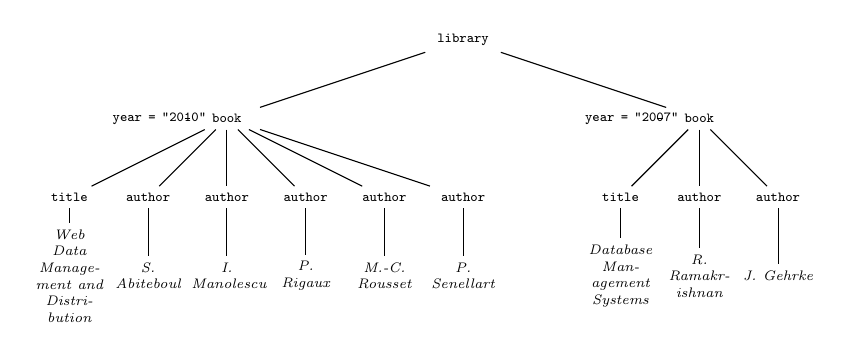
\begin{tikzpicture}[auto]
\tiny
  \tikzstyle{emptyStyle}=[text width=0.9cm, text centered]
  \tikzstyle{red}=[rounded corners=1mm,thick,draw=red!75,fill=red!20,text width=0.9cm, text centered]
  \tikzstyle{DarkViolet}=[rounded corners=1mm,thick,draw=DarkViolet!75,fill=DarkViolet!20,minimum size=7mm,text width=0.8cm, text centered]
  \tikzstyle{green}=[rounded corners=1mm,thick,draw=DarkOliveGreen!75,fill=DarkOliveGreen!20,minimum size=7mm,text width=0.8cm, text centered]
  \tikzstyle{cyan}=[rounded corners=1mm,thick,draw=DarkCyan!75,fill=DarkCyan!20,minimum size=7mm,text width=0.8cm, text centered]
 \tikzstyle{every label}=[black]
  \tikzstyle{HotPink}=[rounded corners=1mm,thick,draw=HotPink!75,fill=HotPink!20,minimum size=7mm,text width=0.8cm, text centered]
  \tikzstyle{Olive}=[rounded corners=1mm,thick,draw=Olive!75,fill=Olive!20,minimum size=7mm,text width=0.9cm, text centered]
  \tikzstyle{indiaRed}=[rounded corners=1mm,thick,draw=indiaRed!75,fill=indiaRed!20,minimum size=7mm,text width=0.9cm, text centered]

  \begin{scope}
   % \node[emptyStyle](r) at (7,5) {Root};  
   %\node[emptyStyle](entete) at (3,4) {\texttt{$<?xml$ version $...>$}};
   %\draw[-] (r) -- (entete);
   \node[emptyStyle](library) at (7,4) {\verb?library?};
   % \draw[-] (r) -- (library);

    \node[emptyStyle](book1) at (4,3) {\verb?book?};
   \draw[-] (library) -- (book1);
   \node[emptyStyle](book2) at (10,3) {\verb?book?};
   \draw[-] (library) -- (book2);

    \node[emptyStyle](year1) at (3,3) {\verb?year = "2010"?};
   \draw[-] (book1) -- (year1);
    \node[emptyStyle](title1) at (2,2) {\verb?title?};
   \draw[-] (book1) -- (title1);
 \node[emptyStyle](texttitle1) at (2,1) {\it Web Data Management and Distribution};
   \draw[-] (title1) -- (texttitle1);
    \node[emptyStyle](author1) at (3,2) {\verb?author?};
   \draw[-] (book1) -- (author1);
   \node[emptyStyle](textauthor1) at (3,1) {\it S. Abiteboul};
   \draw[-] (author1) -- (textauthor1);
    \node[emptyStyle](author2) at (4,2) {\verb?author?};
   \draw[-] (book1) -- (author2);
   \node[emptyStyle](textauthor2) at (4,1) {\it I. Manolescu};
   \draw[-] (author2) -- (textauthor2);
    \node[emptyStyle](author3) at (5,2) {\verb?author?};
   \draw[-] (book1) -- (author3);
   \node[emptyStyle](textauthor3) at (5,1) {\it P. Rigaux};
   \draw[-] (author3) -- (textauthor3);
    \node[emptyStyle](author4) at (6,2) {\verb?author?};
   \draw[-] (book1) -- (author4);
   \node[emptyStyle](textauthor4) at (6,1) {\it M.-C. Rousset};
   \draw[-] (author4) -- (textauthor4);
    \node[emptyStyle](author5) at (7,2) {\verb?author?};
   \draw[-] (book1) -- (author5);
   \node[emptyStyle](textauthor5) at (7,1) {\it P. Senellart};
   \draw[-] (author5) -- (textauthor5);

    \node[emptyStyle](year2) at (9,3) {\verb?year = "2007"?};
   \draw[-] (book2) -- (year2);
    \node[emptyStyle](title2) at (9,2) {\verb?title?};
   \draw[-] (book2) -- (title2);
 \node[emptyStyle](texttitle2) at (9,1) {\it Database Management Systems};
   \draw[-] (title2) -- (texttitle2);
    \node[emptyStyle](author1prime) at (10,2) {\verb?author?};
   \draw[-] (book2) -- (author1prime);
   \node[emptyStyle](textauthor1prime) at (10,1) {\it R. Ramakrishnan};
   \draw[-] (author1prime) -- (textauthor1prime);
    \node[emptyStyle](author2prime) at (11,2) {\verb?author?};
   \draw[-] (book2) -- (author2prime);
   \node[emptyStyle](textauthor2prime) at (11,1) {\it J. Gehrke};
   \draw[-] (author2prime) -- (textauthor2prime);

\end{scope}

\end{tikzpicture}


\end{frame}



\subsection{Child}

\begin{frame}{Quelques axes en exemple : \texttt{child}}

\texttt{child} : tous les enfants du n{\oe}ud courant.

\medskip


\texttt{child} est l'axe par défaut, on peut l'omettre dans les expressions.


\bigskip

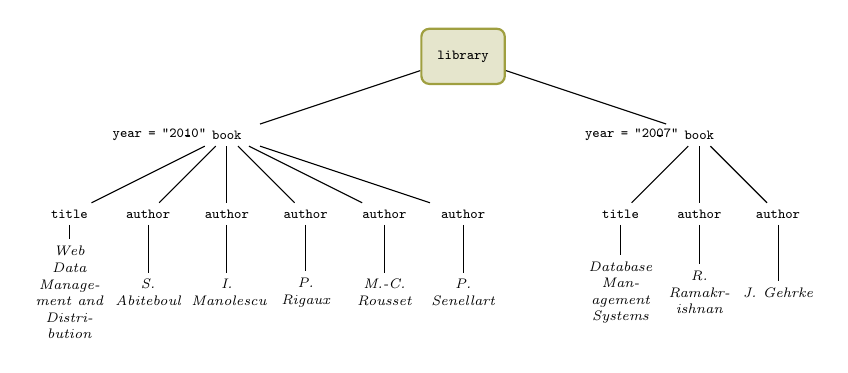
\begin{tikzpicture}[auto]
\tiny
  \tikzstyle{emptyStyle}=[text width=0.9cm, text centered]
  \tikzstyle{red}=[rounded corners=1mm,thick,draw=red!75,fill=red!20,text width=0.9cm, text centered]
  \tikzstyle{DarkViolet}=[rounded corners=1mm,thick,draw=DarkViolet!75,fill=DarkViolet!20,minimum size=7mm,text width=0.8cm, text centered]
  \tikzstyle{green}=[rounded corners=1mm,thick,draw=DarkOliveGreen!75,fill=DarkOliveGreen!20,minimum size=7mm,text width=0.8cm, text centered]
  \tikzstyle{cyan}=[rounded corners=1mm,thick,draw=DarkCyan!75,fill=DarkCyan!20,minimum size=7mm,text width=0.8cm, text centered]
 \tikzstyle{every label}=[black]
  \tikzstyle{HotPink}=[rounded corners=1mm,thick,draw=HotPink!75,fill=HotPink!20,minimum size=7mm,text width=0.8cm, text centered]
  \tikzstyle{noeudcourant}=[rounded corners=1mm,thick,draw=Olive!75,fill=Olive!20,minimum size=7mm,text width=0.9cm, text centered]
  \tikzstyle{indiaRed}=[rounded corners=1mm,thick,draw=indiaRed!75,fill=indiaRed!20,minimum size=7mm,text width=0.9cm, text centered]

  \begin{scope}
   % \node[emptyStyle](r) at (7,5) {Root};  
   %\node[emptyStyle](entete) at (3,4) {\texttt{$<?xml$ version $...>$}};
   %\draw[-] (r) -- (entete);
   \node[noeudcourant](library) at (7,4) {\verb?library?};
   % \draw[-] (r) -- (library);

    \node[emptyStyle](book1) at (4,3) {\verb?book?};
   \draw[-] (library) -- (book1);
   \node[emptyStyle](book2) at (10,3) {\verb?book?};
   \draw[-] (library) -- (book2);

    \node[emptyStyle](year1) at (3,3) {\verb?year = "2010"?};
   \draw[-] (book1) -- (year1);
    \node[emptyStyle](title1) at (2,2) {\verb?title?};
   \draw[-] (book1) -- (title1);
 \node[emptyStyle](texttitle1) at (2,1) {\it Web Data Management and Distribution};
   \draw[-] (title1) -- (texttitle1);
    \node[emptyStyle](author1) at (3,2) {\verb?author?};
   \draw[-] (book1) -- (author1);
   \node[emptyStyle](textauthor1) at (3,1) {\it S. Abiteboul};
   \draw[-] (author1) -- (textauthor1);
    \node[emptyStyle](author2) at (4,2) {\verb?author?};
   \draw[-] (book1) -- (author2);
   \node[emptyStyle](textauthor2) at (4,1) {\it I. Manolescu};
   \draw[-] (author2) -- (textauthor2);
    \node[emptyStyle](author3) at (5,2) {\verb?author?};
   \draw[-] (book1) -- (author3);
   \node[emptyStyle](textauthor3) at (5,1) {\it P. Rigaux};
   \draw[-] (author3) -- (textauthor3);
    \node[emptyStyle](author4) at (6,2) {\verb?author?};
   \draw[-] (book1) -- (author4);
   \node[emptyStyle](textauthor4) at (6,1) {\it M.-C. Rousset};
   \draw[-] (author4) -- (textauthor4);
    \node[emptyStyle](author5) at (7,2) {\verb?author?};
   \draw[-] (book1) -- (author5);
   \node[emptyStyle](textauthor5) at (7,1) {\it P. Senellart};
   \draw[-] (author5) -- (textauthor5);

    \node[emptyStyle](year2) at (9,3) {\verb?year = "2007"?};
   \draw[-] (book2) -- (year2);
    \node[emptyStyle](title2) at (9,2) {\verb?title?};
   \draw[-] (book2) -- (title2);
 \node[emptyStyle](texttitle2) at (9,1) {\it Database Management Systems};
   \draw[-] (title2) -- (texttitle2);
    \node[emptyStyle](author1prime) at (10,2) {\verb?author?};
   \draw[-] (book2) -- (author1prime);
   \node[emptyStyle](textauthor1prime) at (10,1) {\it R. Ramakrishnan};
   \draw[-] (author1prime) -- (textauthor1prime);
    \node[emptyStyle](author2prime) at (11,2) {\verb?author?};
   \draw[-] (book2) -- (author2prime);
   \node[emptyStyle](textauthor2prime) at (11,1) {\it J. Gehrke};
   \draw[-] (author2prime) -- (textauthor2prime);
\end{scope}
\end{tikzpicture}
\end{frame}


\begin{frame}{Quelques axes en exemple : \texttt{child}}
\texttt{child} : tous les enfants du n{\oe}ud courant.


\bigskip

\begin{tikzpicture}[auto]
\tiny
  \tikzstyle{emptyStyle}=[text width=0.9cm, text centered]
  \tikzstyle{red}=[rounded corners=1mm,thick,draw=red!75,fill=red!20,text width=0.9cm, text centered]
  \tikzstyle{DarkViolet}=[rounded corners=1mm,thick,draw=DarkViolet!75,fill=DarkViolet!20,minimum size=7mm,text width=0.8cm, text centered]
  \tikzstyle{green}=[rounded corners=1mm,thick,draw=DarkOliveGreen!75,fill=DarkOliveGreen!20,minimum size=7mm,text width=0.8cm, text centered]
  \tikzstyle{cyan}=[rounded corners=1mm,thick,draw=DarkCyan!75,fill=DarkCyan!20,minimum size=7mm,text width=0.8cm, text centered]
 \tikzstyle{every label}=[black]
  \tikzstyle{HotPink}=[rounded corners=1mm,thick,draw=HotPink!75,fill=HotPink!20,minimum size=7mm,text width=0.8cm, text centered]
  \tikzstyle{noeudcourant}=[rounded corners=1mm,thick,draw=Olive!75,fill=Olive!20,minimum size=7mm,text width=0.9cm, text centered]
  \tikzstyle{indiaRed}=[rounded corners=1mm,thick,draw=indiaRed!75,fill=indiaRed!20,minimum size=7mm,text width=0.9cm, text centered]

  \begin{scope}
   % \node[emptyStyle](r) at (7,5) {Root};  
   %\node[emptyStyle](entete) at (3,4) {\texttt{$<?xml$ version $...>$}};
   %\draw[-] (r) -- (entete);
   \node[noeudcourant](library) at (7,4) {\verb?library?};
   %\draw[-] (r) -- (library);

    \node[indiaRed](book1) at (4,3) {\verb?book?};
   \draw[-] (library) -- (book1);
   \node[indiaRed](book2) at (10,3) {\verb?book?};
   \draw[-] (library) -- (book2);

    \node[emptyStyle](year1) at (3,3) {\verb?year = "2010"?};
   \draw[-] (book1) -- (year1);
    \node[emptyStyle](title1) at (2,2) {\verb?title?};
   \draw[-] (book1) -- (title1);
 \node[emptyStyle](texttitle1) at (2,1) {\it Web Data Management and Distribution};
   \draw[-] (title1) -- (texttitle1);
    \node[emptyStyle](author1) at (3,2) {\verb?author?};
   \draw[-] (book1) -- (author1);
   \node[emptyStyle](textauthor1) at (3,1) {\it S. Abiteboul};
   \draw[-] (author1) -- (textauthor1);
    \node[emptyStyle](author2) at (4,2) {\verb?author?};
   \draw[-] (book1) -- (author2);
   \node[emptyStyle](textauthor2) at (4,1) {\it I. Manolescu};
   \draw[-] (author2) -- (textauthor2);
    \node[emptyStyle](author3) at (5,2) {\verb?author?};
   \draw[-] (book1) -- (author3);
   \node[emptyStyle](textauthor3) at (5,1) {\it P. Rigaux};
   \draw[-] (author3) -- (textauthor3);
    \node[emptyStyle](author4) at (6,2) {\verb?author?};
   \draw[-] (book1) -- (author4);
   \node[emptyStyle](textauthor4) at (6,1) {\it M.-C. Rousset};
   \draw[-] (author4) -- (textauthor4);
    \node[emptyStyle](author5) at (7,2) {\verb?author?};
   \draw[-] (book1) -- (author5);
   \node[emptyStyle](textauthor5) at (7,1) {\it P. Senellart};
   \draw[-] (author5) -- (textauthor5);

    \node[emptyStyle](year2) at (9,3) {\verb?year = "2007"?};
   \draw[-] (book2) -- (year2);
    \node[emptyStyle](title2) at (9,2) {\verb?title?};
   \draw[-] (book2) -- (title2);
 \node[emptyStyle](texttitle2) at (9,1) {\it Database Management Systems};
   \draw[-] (title2) -- (texttitle2);
    \node[emptyStyle](author1prime) at (10,2) {\verb?author?};
   \draw[-] (book2) -- (author1prime);
   \node[emptyStyle](textauthor1prime) at (10,1) {\it R. Ramakrishnan};
   \draw[-] (author1prime) -- (textauthor1prime);
    \node[emptyStyle](author2prime) at (11,2) {\verb?author?};
   \draw[-] (book2) -- (author2prime);
   \node[emptyStyle](textauthor2prime) at (11,1) {\it J. Gehrke};
   \draw[-] (author2prime) -- (textauthor2prime);
\end{scope}
\end{tikzpicture}
\end{frame} 

\begin{frame}{Quelques axes en exemple : \texttt{child}}
\texttt{child} : tous les enfants du n{\oe}ud courant.

\bigskip

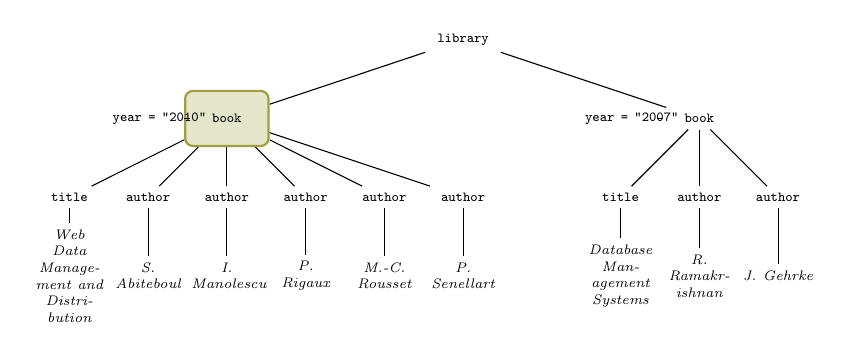
\begin{tikzpicture}[auto]
\tiny
  \tikzstyle{emptyStyle}=[text width=0.9cm, text centered]
  \tikzstyle{red}=[rounded corners=1mm,thick,draw=red!75,fill=red!20,text width=0.9cm, text centered]
  \tikzstyle{DarkViolet}=[rounded corners=1mm,thick,draw=DarkViolet!75,fill=DarkViolet!20,minimum size=7mm,text width=0.8cm, text centered]
  \tikzstyle{green}=[rounded corners=1mm,thick,draw=DarkOliveGreen!75,fill=DarkOliveGreen!20,minimum size=7mm,text width=0.8cm, text centered]
  \tikzstyle{cyan}=[rounded corners=1mm,thick,draw=DarkCyan!75,fill=DarkCyan!20,minimum size=7mm,text width=0.8cm, text centered]
 \tikzstyle{every label}=[black]
  \tikzstyle{HotPink}=[rounded corners=1mm,thick,draw=HotPink!75,fill=HotPink!20,minimum size=7mm,text width=0.8cm, text centered]
  \tikzstyle{noeudcourant}=[rounded corners=1mm,thick,draw=Olive!75,fill=Olive!20,minimum size=7mm,text width=0.9cm, text centered]
  \tikzstyle{indiaRed}=[rounded corners=1mm,thick,draw=indiaRed!75,fill=indiaRed!20,minimum size=7mm,text width=0.9cm, text centered]

  \begin{scope}
   % \node[emptyStyle](r) at (7,5) {Root};  
   %\node[emptyStyle](entete) at (3,4) {\texttt{$<?xml$ version $...>$}};
   %\draw[-] (r) -- (entete);
   \node[emptyStyle](library) at (7,4) {\verb?library?};
   % \draw[-] (r) -- (library);

    \node[noeudcourant](book1) at (4,3) {\verb?book?};
   \draw[-] (library) -- (book1);
   \node[emptyStyle](book2) at (10,3) {\verb?book?};
   \draw[-] (library) -- (book2);

    \node[emptyStyle](year1) at (3,3) {\verb?year = "2010"?};
   \draw[-] (book1) -- (year1);
    \node[emptyStyle](title1) at (2,2) {\verb?title?};
   \draw[-] (book1) -- (title1);
 \node[emptyStyle](texttitle1) at (2,1) {\it Web Data Management and Distribution};
   \draw[-] (title1) -- (texttitle1);
    \node[emptyStyle](author1) at (3,2) {\verb?author?};
   \draw[-] (book1) -- (author1);
   \node[emptyStyle](textauthor1) at (3,1) {\it S. Abiteboul};
   \draw[-] (author1) -- (textauthor1);
    \node[emptyStyle](author2) at (4,2) {\verb?author?};
   \draw[-] (book1) -- (author2);
   \node[emptyStyle](textauthor2) at (4,1) {\it I. Manolescu};
   \draw[-] (author2) -- (textauthor2);
    \node[emptyStyle](author3) at (5,2) {\verb?author?};
   \draw[-] (book1) -- (author3);
   \node[emptyStyle](textauthor3) at (5,1) {\it P. Rigaux};
   \draw[-] (author3) -- (textauthor3);
    \node[emptyStyle](author4) at (6,2) {\verb?author?};
   \draw[-] (book1) -- (author4);
   \node[emptyStyle](textauthor4) at (6,1) {\it M.-C. Rousset};
   \draw[-] (author4) -- (textauthor4);
    \node[emptyStyle](author5) at (7,2) {\verb?author?};
   \draw[-] (book1) -- (author5);
   \node[emptyStyle](textauthor5) at (7,1) {\it P. Senellart};
   \draw[-] (author5) -- (textauthor5);

    \node[emptyStyle](year2) at (9,3) {\verb?year = "2007"?};
   \draw[-] (book2) -- (year2);
    \node[emptyStyle](title2) at (9,2) {\verb?title?};
   \draw[-] (book2) -- (title2);
 \node[emptyStyle](texttitle2) at (9,1) {\it Database Management Systems};
   \draw[-] (title2) -- (texttitle2);
    \node[emptyStyle](author1prime) at (10,2) {\verb?author?};
   \draw[-] (book2) -- (author1prime);
   \node[emptyStyle](textauthor1prime) at (10,1) {\it R. Ramakrishnan};
   \draw[-] (author1prime) -- (textauthor1prime);
    \node[emptyStyle](author2prime) at (11,2) {\verb?author?};
   \draw[-] (book2) -- (author2prime);
   \node[emptyStyle](textauthor2prime) at (11,1) {\it J. Gehrke};
   \draw[-] (author2prime) -- (textauthor2prime);
\end{scope}
\end{tikzpicture}
\end{frame}


\begin{frame}{Quelques axes en exemple : \texttt{child}}
\texttt{child} : tous les enfants du n{\oe}ud courant.

\bigskip

\begin{tikzpicture}[auto]
\tiny
  \tikzstyle{emptyStyle}=[text width=0.9cm, text centered]
  \tikzstyle{red}=[rounded corners=1mm,thick,draw=red!75,fill=red!20,text width=0.9cm, text centered]
  \tikzstyle{DarkViolet}=[rounded corners=1mm,thick,draw=DarkViolet!75,fill=DarkViolet!20,minimum size=7mm,text width=0.8cm, text centered]
  \tikzstyle{green}=[rounded corners=1mm,thick,draw=DarkOliveGreen!75,fill=DarkOliveGreen!20,minimum size=7mm,text width=0.8cm, text centered]
  \tikzstyle{cyan}=[rounded corners=1mm,thick,draw=DarkCyan!75,fill=DarkCyan!20,minimum size=7mm,text width=0.8cm, text centered]
 \tikzstyle{every label}=[black]
  \tikzstyle{HotPink}=[rounded corners=1mm,thick,draw=HotPink!75,fill=HotPink!20,minimum size=7mm,text width=0.8cm, text centered]
  \tikzstyle{noeudcourant}=[rounded corners=1mm,thick,draw=Olive!75,fill=Olive!20,minimum size=7mm,text width=0.9cm, text centered]
  \tikzstyle{indiaRed}=[rounded corners=1mm,thick,draw=indiaRed!75,fill=indiaRed!20,minimum size=7mm,text width=0.9cm, text centered]

  \begin{scope}
   % \node[emptyStyle](r) at (7,5) {Root};  
   %\node[emptyStyle](entete) at (3,4) {\texttt{$<?xml$ version $...>$}};
   %\draw[-] (r) -- (entete);
   \node[emptyStyle](library) at (7,4) {\verb?library?};
   % \draw[-] (r) -- (library);

    \node[noeudcourant](book1) at (4,3) {\verb?book?};
   \draw[-] (library) -- (book1);
   \node[emptyStyle](book2) at (10,3) {\verb?book?};
   \draw[-] (library) -- (book2);

    \node[emptyStyle](year1) at (3,3) {\verb?year = "2010"?};
   \draw[-] (book1) -- (year1);
    \node[indiaRed](title1) at (2,2) {\verb?title?};
   \draw[-] (book1) -- (title1);
 \node[emptyStyle](texttitle1) at (2,1) {\it Web Data Management and Distribution};
   \draw[-] (title1) -- (texttitle1);
    \node[indiaRed](author1) at (3,2) {\verb?author?};
   \draw[-] (book1) -- (author1);
   \node[emptyStyle](textauthor1) at (3,1) {\it S. Abiteboul};
   \draw[-] (author1) -- (textauthor1);
    \node[indiaRed](author2) at (4,2) {\verb?author?};
   \draw[-] (book1) -- (author2);
   \node[emptyStyle](textauthor2) at (4,1) {\it I. Manolescu};
   \draw[-] (author2) -- (textauthor2);
    \node[indiaRed](author3) at (5,2) {\verb?author?};
   \draw[-] (book1) -- (author3);
   \node[emptyStyle](textauthor3) at (5,1) {\it P. Rigaux};
   \draw[-] (author3) -- (textauthor3);
    \node[indiaRed](author4) at (6,2) {\verb?author?};
   \draw[-] (book1) -- (author4);
   \node[emptyStyle](textauthor4) at (6,1) {\it M.-C. Rousset};
   \draw[-] (author4) -- (textauthor4);
    \node[indiaRed](author5) at (7,2) {\verb?author?};
   \draw[-] (book1) -- (author5);
   \node[emptyStyle](textauthor5) at (7,1) {\it P. Senellart};
   \draw[-] (author5) -- (textauthor5);

    \node[emptyStyle](year2) at (9,3) {\verb?year = "2007"?};
   \draw[-] (book2) -- (year2);
    \node[emptyStyle](title2) at (9,2) {\verb?title?};
   \draw[-] (book2) -- (title2);
 \node[emptyStyle](texttitle2) at (9,1) {\it Database Management Systems};
   \draw[-] (title2) -- (texttitle2);
    \node[emptyStyle](author1prime) at (10,2) {\verb?author?};
   \draw[-] (book2) -- (author1prime);
   \node[emptyStyle](textauthor1prime) at (10,1) {\it R. Ramakrishnan};
   \draw[-] (author1prime) -- (textauthor1prime);
    \node[emptyStyle](author2prime) at (11,2) {\verb?author?};
   \draw[-] (book2) -- (author2prime);
   \node[emptyStyle](textauthor2prime) at (11,1) {\it J. Gehrke};
   \draw[-] (author2prime) -- (textauthor2prime);
\end{scope}
\end{tikzpicture}
\end{frame}


\subsection{Attribute}
%attribute

 \begin{frame}{Quelques axes en exemple : \texttt{attribute}}
\texttt{attribute} : sélectionne les attributs du n{\oe}ud courant.

\medskip

\texttt{attribute} peut s'abréger en "@".

\medskip

Un attribut n'est pas un enfant de son n{\oe}ud élément.

\bigskip

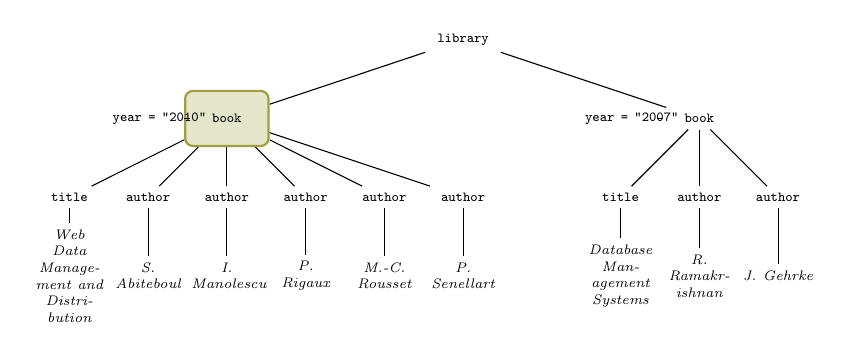
\begin{tikzpicture}[auto]
\tiny
  \tikzstyle{emptyStyle}=[text width=0.9cm, text centered]
  \tikzstyle{red}=[rounded corners=1mm,thick,draw=red!75,fill=red!20,text width=0.9cm, text centered]
  \tikzstyle{DarkViolet}=[rounded corners=1mm,thick,draw=DarkViolet!75,fill=DarkViolet!20,minimum size=7mm,text width=0.8cm, text centered]
  \tikzstyle{green}=[rounded corners=1mm,thick,draw=DarkOliveGreen!75,fill=DarkOliveGreen!20,minimum size=7mm,text width=0.8cm, text centered]
  \tikzstyle{cyan}=[rounded corners=1mm,thick,draw=DarkCyan!75,fill=DarkCyan!20,minimum size=7mm,text width=0.8cm, text centered]
 \tikzstyle{every label}=[black]
  \tikzstyle{HotPink}=[rounded corners=1mm,thick,draw=HotPink!75,fill=HotPink!20,minimum size=7mm,text width=0.8cm, text centered]
  \tikzstyle{noeudcourant}=[rounded corners=1mm,thick,draw=Olive!75,fill=Olive!20,minimum size=7mm,text width=0.9cm, text centered]
  \tikzstyle{indiaRed}=[rounded corners=1mm,thick,draw=indiaRed!75,fill=indiaRed!20,minimum size=7mm,text width=0.9cm, text centered]

  \begin{scope}
   % \node[emptyStyle](r) at (7,5) {Root};  
   %\node[emptyStyle](entete) at (3,4) {\texttt{$<?xml$ version $...>$}};
   %\draw[-] (r) -- (entete);
   \node[emptyStyle](library) at (7,4) {\verb?library?};
   % \draw[-] (r) -- (library);

    \node[noeudcourant](book1) at (4,3) {\verb?book?};
   \draw[-] (library) -- (book1);
   \node[emptyStyle](book2) at (10,3) {\verb?book?};
   \draw[-] (library) -- (book2);

    \node[emptyStyle](year1) at (3,3) {\verb?year = "2010"?};
   \draw[-] (book1) -- (year1);
    \node[emptyStyle](title1) at (2,2) {\verb?title?};
   \draw[-] (book1) -- (title1);
 \node[emptyStyle](texttitle1) at (2,1) {\it Web Data Management and Distribution};
   \draw[-] (title1) -- (texttitle1);
    \node[emptyStyle](author1) at (3,2) {\verb?author?};
   \draw[-] (book1) -- (author1);
   \node[emptyStyle](textauthor1) at (3,1) {\it S. Abiteboul};
   \draw[-] (author1) -- (textauthor1);
    \node[emptyStyle](author2) at (4,2) {\verb?author?};
   \draw[-] (book1) -- (author2);
   \node[emptyStyle](textauthor2) at (4,1) {\it I. Manolescu};
   \draw[-] (author2) -- (textauthor2);
    \node[emptyStyle](author3) at (5,2) {\verb?author?};
   \draw[-] (book1) -- (author3);
   \node[emptyStyle](textauthor3) at (5,1) {\it P. Rigaux};
   \draw[-] (author3) -- (textauthor3);
    \node[emptyStyle](author4) at (6,2) {\verb?author?};
   \draw[-] (book1) -- (author4);
   \node[emptyStyle](textauthor4) at (6,1) {\it M.-C. Rousset};
   \draw[-] (author4) -- (textauthor4);
    \node[emptyStyle](author5) at (7,2) {\verb?author?};
   \draw[-] (book1) -- (author5);
   \node[emptyStyle](textauthor5) at (7,1) {\it P. Senellart};
   \draw[-] (author5) -- (textauthor5);

    \node[emptyStyle](year2) at (9,3) {\verb?year = "2007"?};
   \draw[-] (book2) -- (year2);
    \node[emptyStyle](title2) at (9,2) {\verb?title?};
   \draw[-] (book2) -- (title2);
 \node[emptyStyle](texttitle2) at (9,1) {\it Database Management Systems};
   \draw[-] (title2) -- (texttitle2);
    \node[emptyStyle](author1prime) at (10,2) {\verb?author?};
   \draw[-] (book2) -- (author1prime);
   \node[emptyStyle](textauthor1prime) at (10,1) {\it R. Ramakrishnan};
   \draw[-] (author1prime) -- (textauthor1prime);
    \node[emptyStyle](author2prime) at (11,2) {\verb?author?};
   \draw[-] (book2) -- (author2prime);
   \node[emptyStyle](textauthor2prime) at (11,1) {\it J. Gehrke};
   \draw[-] (author2prime) -- (textauthor2prime);
\end{scope}
\end{tikzpicture}




\end{frame}


 \begin{frame}{Quelques axes en exemple : \texttt{attribute}}
\texttt{attribute} : sélectionne les attributs du n{\oe}ud courant.


\bigskip

\begin{tikzpicture}[auto]
\tiny
  \tikzstyle{emptyStyle}=[text width=0.9cm, text centered]
  \tikzstyle{red}=[rounded corners=1mm,thick,draw=red!75,fill=red!20,text width=0.9cm, text centered]
  \tikzstyle{DarkViolet}=[rounded corners=1mm,thick,draw=DarkViolet!75,fill=DarkViolet!20,minimum size=7mm,text width=0.8cm, text centered]
  \tikzstyle{green}=[rounded corners=1mm,thick,draw=DarkOliveGreen!75,fill=DarkOliveGreen!20,minimum size=7mm,text width=0.8cm, text centered]
  \tikzstyle{cyan}=[rounded corners=1mm,thick,draw=DarkCyan!75,fill=DarkCyan!20,minimum size=7mm,text width=0.8cm, text centered]
 \tikzstyle{every label}=[black]
  \tikzstyle{HotPink}=[rounded corners=1mm,thick,draw=HotPink!75,fill=HotPink!20,minimum size=7mm,text width=0.8cm, text centered]
  \tikzstyle{noeudcourant}=[rounded corners=1mm,thick,draw=Olive!75,fill=Olive!20,minimum size=7mm,text width=0.9cm, text centered]
  \tikzstyle{indiaRed}=[rounded corners=1mm,thick,draw=indiaRed!75,fill=indiaRed!20,minimum size=7mm,text width=0.9cm, text centered]

  \begin{scope}
   % \node[emptyStyle](r) at (7,5) {Root};  
   %\node[emptyStyle](entete) at (3,4) {\texttt{$<?xml$ version $...>$}};
   %\draw[-] (r) -- (entete);
   \node[emptyStyle](library) at (7,4) {\verb?library?};
   % \draw[-] (r) -- (library);

    \node[noeudcourant](book1) at (4,3) {\verb?book?};
   \draw[-] (library) -- (book1);
   \node[emptyStyle](book2) at (10,3) {\verb?book?};
   \draw[-] (library) -- (book2);

    \node[indiaRed](year1) at (3,3) {\verb?year = "2010"?};
   \draw[-] (book1) -- (year1);
    \node[emptyStyle](title1) at (2,2) {\verb?title?};
   \draw[-] (book1) -- (title1);
 \node[emptyStyle](texttitle1) at (2,1) {\it Web Data Management and Distribution};
   \draw[-] (title1) -- (texttitle1);
    \node[emptyStyle](author1) at (3,2) {\verb?author?};
   \draw[-] (book1) -- (author1);
   \node[emptyStyle](textauthor1) at (3,1) {\it S. Abiteboul};
   \draw[-] (author1) -- (textauthor1);
    \node[emptyStyle](author2) at (4,2) {\verb?author?};
   \draw[-] (book1) -- (author2);
   \node[emptyStyle](textauthor2) at (4,1) {\it I. Manolescu};
   \draw[-] (author2) -- (textauthor2);
    \node[emptyStyle](author3) at (5,2) {\verb?author?};
   \draw[-] (book1) -- (author3);
   \node[emptyStyle](textauthor3) at (5,1) {\it P. Rigaux};
   \draw[-] (author3) -- (textauthor3);
    \node[emptyStyle](author4) at (6,2) {\verb?author?};
   \draw[-] (book1) -- (author4);
   \node[emptyStyle](textauthor4) at (6,1) {\it M.-C. Rousset};
   \draw[-] (author4) -- (textauthor4);
    \node[emptyStyle](author5) at (7,2) {\verb?author?};
   \draw[-] (book1) -- (author5);
   \node[emptyStyle](textauthor5) at (7,1) {\it P. Senellart};
   \draw[-] (author5) -- (textauthor5);

    \node[emptyStyle](year2) at (9,3) {\verb?year = "2007"?};
   \draw[-] (book2) -- (year2);
    \node[emptyStyle](title2) at (9,2) {\verb?title?};
   \draw[-] (book2) -- (title2);
 \node[emptyStyle](texttitle2) at (9,1) {\it Database Management Systems};
   \draw[-] (title2) -- (texttitle2);
    \node[emptyStyle](author1prime) at (10,2) {\verb?author?};
   \draw[-] (book2) -- (author1prime);
   \node[emptyStyle](textauthor1prime) at (10,1) {\it R. Ramakrishnan};
   \draw[-] (author1prime) -- (textauthor1prime);
    \node[emptyStyle](author2prime) at (11,2) {\verb?author?};
   \draw[-] (book2) -- (author2prime);
   \node[emptyStyle](textauthor2prime) at (11,1) {\it J. Gehrke};
   \draw[-] (author2prime) -- (textauthor2prime);
\end{scope}
\end{tikzpicture}

\end{frame}



\begin{frame}[allowframebreaks]{Exemple}

%\begin{center}
%\begin{minipage}{0.7\textwidth}
%\lstinputlisting[basicstyle=\tiny, language=XML,breaklines=true, caption={Un simple fichier XML}]{codes/livresExXpath.xml}
%\end{minipage}
%\end{center}

%\framebreak

\texttt{/child::library/child::*/@year}

\medskip

S'abrège en\,: \texttt{/library/*/@year}

\begin{center}
\begin{tikzpicture}[auto]
\tiny
  \tikzstyle{emptyStyle}=[text width=0.9cm, text centered]
  \tikzstyle{parser}=[rounded corners=3mm,thick,draw=DarkViolet!75,fill=DarkViolet!20,,text centered]
  \tikzstyle{appli}=[rounded corners=1mm,thick,draw=red!75,fill=red!20,text centered,text width=2cm]
  \tikzstyle{every label}=[black]

  \begin{scope}
    \node[emptyStyle](r) at (6,5) {Root};
   \node[emptyStyle](comment) at (1,4) {\texttt{\verb?<!-- ceci ... >?}};
   \draw[-] (r) -- (comment);
    %\node[emptyStyle](entete) at (3,4) {\texttt{$<?xml$ version $...>$}};
   %\draw[-] (r) -- (entete);
    \node[emptyStyle](library) at (6,4) {\verb?<library> ... </library>?};
   \draw[-] (r) -- (library);

    \node[emptyStyle](book1) at (3,3) {\verb?<book> ... </book>?};
   \draw[-] (library) -- (book1);
    \node[emptyStyle](book2) at (6,3) {\verb?<book> ... </book>?};
   \draw[-] (library) -- (book2);
    \node[emptyStyle](book3) at (10,3) {\verb?<book> ... </book>?};
   \draw[-] (library) -- (book3);

    \node[emptyStyle](year1) at (2,3) {\verb?year = "1857"?};
   \draw[-] (book1) -- (year1);
    \node[emptyStyle](author1) at (2,2) {\verb?<author> ... </author>?};
   \draw[-] (book1) -- (author1);
    \node[emptyStyle](textauthor1) at (2,1) {\it Charles Baudelaire};
   \draw[-] (author1) -- (textauthor1);
    \node[emptyStyle](title1) at (3,2) {\verb?<title> ... </title>?};
   \draw[-] (book1) -- (title1);
    \node[emptyStyle](texttitle1) at (3,1) {\it Les fleurs du mal};
   \draw[-] (title1) -- (texttitle1);

    \node[emptyStyle](year2) at (5,3) {\verb?year = "1862"?};
   \draw[-] (book2) -- (year2);
    \node[emptyStyle](author2) at (6,2) {\verb?<author> ... </author>?};
   \draw[-] (book2) -- (author2);
    \node[emptyStyle](textauthor2) at (6,1) {\it Victor Hugo};
   \draw[-] (author2) -- (textauthor2);
    \node[emptyStyle](ln2) at (5,2) {\verb?ln = "Besancon"?};
   \draw[-] (author2) -- (ln2);
    \node[emptyStyle](title2) at (7,2) {\verb?<title> ... </title>?};
   \draw[-] (book2) -- (title2);
    \node[emptyStyle](texttitle2) at (7,1) {\it Les miserables};
   \draw[-] (title2) -- (texttitle2);

    \node[emptyStyle](year3) at (9,3) {\verb?year = "1877"?};
   \draw[-] (book3) -- (year3);
    \node[emptyStyle](author3) at (10,2) {\verb?<author> ... </author>?};
   \draw[-] (book3) -- (author3);
    \node[emptyStyle](textauthor3) at (10,1) {\it Emile Zola};
   \draw[-] (author3) -- (textauthor3);
    \node[emptyStyle](ln3) at (9,2) {\verb?ln = "Paris"?};
   \draw[-] (author3) -- (ln3);
    \node[emptyStyle](title3) at (11,2) {\verb?<title> ... </title>?};
   \draw[-] (book3) -- (title3);
    \node[emptyStyle](texttitle3) at (11,1) {\it L'assomoir};
   \draw[-] (title3) -- (texttitle3);

\end{scope}

%  \begin{pgfonlayer}{background}
%    \filldraw [line width=4mm,join=round,black!20]
%      (parser.north  -| parser.west)  rectangle (serial.south  -| serial.east);
%\end{pgfonlayer}


\end{tikzpicture}
\end{center}

\framebreak

\texttt{\textcolor{red}{\bf /}library/*/@year}

\begin{center}
\begin{tikzpicture}[auto]
\tiny
  \tikzstyle{emptyStyle}=[text width=0.9cm, text centered]
  \tikzstyle{red}=[rounded corners=1mm,thick,draw=red!75,fill=red!20,text width=0.9cm, text centered]
  \tikzstyle{DarkViolet}=[rounded corners=1mm,thick,draw=DarkViolet!75,fill=DarkViolet!20,minimum size=7mm,text width=0.8cm, text centered]
 \tikzstyle{every label}=[black]

  \begin{scope}
    \node[red](r) at (6,5) {Root};
   \node[emptyStyle](comment) at (1,4) {\texttt{\verb?<!-- ceci ... >?}};
   \draw[-] (r) -- (comment);
    %\node[emptyStyle](entete) at (3,4) {\texttt{$<?xml$ version $...>$}};
   %\draw[-] (r) -- (entete);
    \node[emptyStyle](library) at (6,4) {\verb?<library> ... </library>?};
   \draw[-] (r) -- (library);

    \node[emptyStyle](book1) at (3,3) {\verb?<book> ... </book>?};
   \draw[-] (library) -- (book1);
    \node[emptyStyle](book2) at (6,3) {\verb?<book> ... </book>?};
   \draw[-] (library) -- (book2);
    \node[emptyStyle](book3) at (10,3) {\verb?<book> ... </book>?};
   \draw[-] (library) -- (book3);

    \node[emptyStyle](year1) at (2,3) {\verb?year = "1857"?};
   \draw[-] (book1) -- (year1);
    \node[emptyStyle](author1) at (2,2) {\verb?<author> ... </author>?};
   \draw[-] (book1) -- (author1);
    \node[emptyStyle](textauthor1) at (2,1) {\it Charles Baudelaire};
   \draw[-] (author1) -- (textauthor1);
    \node[emptyStyle](title1) at (3,2) {\verb?<title> ... </title>?};
   \draw[-] (book1) -- (title1);
    \node[emptyStyle](texttitle1) at (3,1) {\it Les fleurs du mal};
   \draw[-] (title1) -- (texttitle1);

    \node[emptyStyle](year2) at (5,3) {\verb?year = "1862"?};
   \draw[-] (book2) -- (year2);
    \node[emptyStyle](author2) at (6,2) {\verb?<author> ... </author>?};
   \draw[-] (book2) -- (author2);
    \node[emptyStyle](textauthor2) at (6,1) {\it Victor Hugo};
   \draw[-] (author2) -- (textauthor2);
    \node[emptyStyle](ln2) at (5,2) {\verb?ln = "Besancon"?};
   \draw[-] (author2) -- (ln2);
    \node[emptyStyle](title2) at (7,2) {\verb?<title> ... </title>?};
   \draw[-] (book2) -- (title2);
    \node[emptyStyle](texttitle2) at (7,1) {\it Les miserables};
   \draw[-] (title2) -- (texttitle2);

    \node[emptyStyle](year3) at (9,3) {\verb?year = "1877"?};
   \draw[-] (book3) -- (year3);
    \node[emptyStyle](author3) at (10,2) {\verb?<author> ... </author>?};
   \draw[-] (book3) -- (author3);
    \node[emptyStyle](textauthor3) at (10,1) {\it Emile Zola};
   \draw[-] (author3) -- (textauthor3);
    \node[emptyStyle](ln3) at (9,2) {\verb?ln = "Paris"?};
   \draw[-] (author3) -- (ln3);
    \node[emptyStyle](title3) at (11,2) {\verb?<title> ... </title>?};
   \draw[-] (book3) -- (title3);
    \node[emptyStyle](texttitle3) at (11,1) {\it L'assomoir};
   \draw[-] (title3) -- (texttitle3);

\end{scope}

%  \begin{pgfonlayer}{background}
%    \filldraw [line width=4mm,join=round,black!20]
%      (parser.north  -| parser.west)  rectangle (serial.south  -| serial.east);
%\end{pgfonlayer}


\end{tikzpicture}
\end{center}


\framebreak

\texttt{\textcolor{red}{\bf /}\textcolor{DarkViolet}{\bf library}/*/@year}

\begin{center}
\begin{tikzpicture}[auto]
\tiny
  \tikzstyle{emptyStyle}=[text width=0.9cm, text centered]
  \tikzstyle{red}=[rounded corners=1mm,thick,draw=red!75,fill=red!20,text width=0.9cm, text centered]
  \tikzstyle{DarkViolet}=[rounded corners=1mm,thick,draw=DarkViolet!75,fill=DarkViolet!20,minimum size=7mm,text width=0.8cm, text centered]
 \tikzstyle{every label}=[black]

  \begin{scope}
    \node[red](r) at (6,5) {Root};
   \node[emptyStyle](comment) at (1,4) {\texttt{\verb?<!-- ceci ... >?}};
   \draw[-] (r) -- (comment);
    %\node[emptyStyle](entete) at (3,4) {\texttt{$<?xml$ version $...>$}};
   %\draw[-] (r) -- (entete);
    \node[DarkViolet](library) at (6,4) {\verb?<library> ... </library>?};
   \draw[-] (r) -- (library);

    \node[emptyStyle](book1) at (3,3) {\verb?<book> ... </book>?};
   \draw[-] (library) -- (book1);
    \node[emptyStyle](book2) at (6,3) {\verb?<book> ... </book>?};
   \draw[-] (library) -- (book2);
    \node[emptyStyle](book3) at (10,3) {\verb?<book> ... </book>?};
   \draw[-] (library) -- (book3);

    \node[emptyStyle](year1) at (2,3) {\verb?year = "1857"?};
   \draw[-] (book1) -- (year1);
    \node[emptyStyle](author1) at (2,2) {\verb?<author> ... </author>?};
   \draw[-] (book1) -- (author1);
    \node[emptyStyle](textauthor1) at (2,1) {\it Charles Baudelaire};
   \draw[-] (author1) -- (textauthor1);
    \node[emptyStyle](title1) at (3,2) {\verb?<title> ... </title>?};
   \draw[-] (book1) -- (title1);
    \node[emptyStyle](texttitle1) at (3,1) {\it Les fleurs du mal};
   \draw[-] (title1) -- (texttitle1);

    \node[emptyStyle](year2) at (5,3) {\verb?year = "1862"?};
   \draw[-] (book2) -- (year2);
    \node[emptyStyle](author2) at (6,2) {\verb?<author> ... </author>?};
   \draw[-] (book2) -- (author2);
    \node[emptyStyle](textauthor2) at (6,1) {\it Victor Hugo};
   \draw[-] (author2) -- (textauthor2);
    \node[emptyStyle](ln2) at (5,2) {\verb?ln = "Besancon"?};
   \draw[-] (author2) -- (ln2);
    \node[emptyStyle](title2) at (7,2) {\verb?<title> ... </title>?};
   \draw[-] (book2) -- (title2);
    \node[emptyStyle](texttitle2) at (7,1) {\it Les miserables};
   \draw[-] (title2) -- (texttitle2);

    \node[emptyStyle](year3) at (9,3) {\verb?year = "1877"?};
   \draw[-] (book3) -- (year3);
    \node[emptyStyle](author3) at (10,2) {\verb?<author> ... </author>?};
   \draw[-] (book3) -- (author3);
    \node[emptyStyle](textauthor3) at (10,1) {\it Emile Zola};
   \draw[-] (author3) -- (textauthor3);
    \node[emptyStyle](ln3) at (9,2) {\verb?ln = "Paris"?};
   \draw[-] (author3) -- (ln3);
    \node[emptyStyle](title3) at (11,2) {\verb?<title> ... </title>?};
   \draw[-] (book3) -- (title3);
    \node[emptyStyle](texttitle3) at (11,1) {\it L'assomoir};
   \draw[-] (title3) -- (texttitle3);

\end{scope}

%  \begin{pgfonlayer}{background}
%    \filldraw [line width=4mm,join=round,black!20]
%      (parser.north  -| parser.west)  rectangle (serial.south  -| serial.east);
%\end{pgfonlayer}


\end{tikzpicture}
\end{center}

\framebreak

\texttt{\textcolor{red}{\bf /}\textcolor{DarkViolet}{\bf library}\textcolor{DarkOliveGreen}{\bf /*}/@year}

\begin{center}
\begin{tikzpicture}[auto]
\tiny
  \tikzstyle{emptyStyle}=[text width=0.9cm, text centered]
  \tikzstyle{red}=[rounded corners=1mm,thick,draw=red!75,fill=red!20,text width=0.9cm, text centered]
  \tikzstyle{DarkViolet}=[rounded corners=1mm,thick,draw=DarkViolet!75,fill=DarkViolet!20,minimum size=7mm,text width=0.8cm, text centered]
  \tikzstyle{green}=[rounded corners=1mm,thick,draw=DarkOliveGreen!75,fill=DarkOliveGreen!20,minimum size=7mm,text width=0.8cm, text centered]
 \tikzstyle{every label}=[black]

  \begin{scope}
    \node[red](r) at (6,5) {Root};
   \node[emptyStyle](comment) at (1,4) {\texttt{\verb?<!-- ceci ... >?}};
   \draw[-] (r) -- (comment);
    %\node[emptyStyle](entete) at (3,4) {\texttt{$<?xml$ version $...>$}};
   %\draw[-] (r) -- (entete);
    \node[DarkViolet](library) at (6,4) {\verb?<library> ... </library>?};
   \draw[-] (r) -- (library);

    \node[green](book1) at (3,3) {\verb?<book> ... </book>?};
   \draw[-] (library) -- (book1);
    \node[green](book2) at (6,3) {\verb?<book> ... </book>?};
   \draw[-] (library) -- (book2);
    \node[green](book3) at (10,3) {\verb?<book> ... </book>?};
   \draw[-] (library) -- (book3);

    \node[emptyStyle](year1) at (2,3) {\verb?year = "1857"?};
   \draw[-] (book1) -- (year1);
    \node[emptyStyle](author1) at (2,2) {\verb?<author> ... </author>?};
   \draw[-] (book1) -- (author1);
    \node[emptyStyle](textauthor1) at (2,1) {\it Charles Baudelaire};
   \draw[-] (author1) -- (textauthor1);
    \node[emptyStyle](title1) at (3,2) {\verb?<title> ... </title>?};
   \draw[-] (book1) -- (title1);
    \node[emptyStyle](texttitle1) at (3,1) {\it Les fleurs du mal};
   \draw[-] (title1) -- (texttitle1);

    \node[emptyStyle](year2) at (5,3) {\verb?year = "1862"?};
   \draw[-] (book2) -- (year2);
    \node[emptyStyle](author2) at (6,2) {\verb?<author> ... </author>?};
   \draw[-] (book2) -- (author2);
    \node[emptyStyle](textauthor2) at (6,1) {\it Victor Hugo};
   \draw[-] (author2) -- (textauthor2);
    \node[emptyStyle](ln2) at (5,2) {\verb?ln = "Besancon"?};
   \draw[-] (author2) -- (ln2);
    \node[emptyStyle](title2) at (7,2) {\verb?<title> ... </title>?};
   \draw[-] (book2) -- (title2);
    \node[emptyStyle](texttitle2) at (7,1) {\it Les miserables};
   \draw[-] (title2) -- (texttitle2);

    \node[emptyStyle](year3) at (9,3) {\verb?year = "1877"?};
   \draw[-] (book3) -- (year3);
    \node[emptyStyle](author3) at (10,2) {\verb?<author> ... </author>?};
   \draw[-] (book3) -- (author3);
    \node[emptyStyle](textauthor3) at (10,1) {\it Emile Zola};
   \draw[-] (author3) -- (textauthor3);
    \node[emptyStyle](ln3) at (9,2) {\verb?ln = "Paris"?};
   \draw[-] (author3) -- (ln3);
    \node[emptyStyle](title3) at (11,2) {\verb?<title> ... </title>?};
   \draw[-] (book3) -- (title3);
    \node[emptyStyle](texttitle3) at (11,1) {\it L'assomoir};
   \draw[-] (title3) -- (texttitle3);

\end{scope}

%  \begin{pgfonlayer}{background}
%    \filldraw [line width=4mm,join=round,black!20]
%      (parser.north  -| parser.west)  rectangle (serial.south  -| serial.east);
%\end{pgfonlayer}


\end{tikzpicture}
\end{center}


\framebreak

\texttt{\textcolor{red}{\bf /}\textcolor{DarkViolet}{\bf library}\textcolor{DarkOliveGreen}{\bf /*}\textcolor{DarkCyan}{\bf  /@year}}


\begin{center}
\begin{tikzpicture}[auto]
\tiny
  \tikzstyle{emptyStyle}=[text width=0.9cm, text centered]
  \tikzstyle{red}=[rounded corners=1mm,thick,draw=red!75,fill=red!20,text width=0.9cm, text centered]
  \tikzstyle{DarkViolet}=[rounded corners=1mm,thick,draw=DarkViolet!75,fill=DarkViolet!20,minimum size=7mm,text width=0.8cm, text centered]
  \tikzstyle{green}=[rounded corners=1mm,thick,draw=DarkOliveGreen!75,fill=DarkOliveGreen!20,minimum size=7mm,text width=0.8cm, text centered]
  \tikzstyle{cyan}=[rounded corners=1mm,thick,draw=DarkCyan!75,fill=DarkCyan!20,minimum size=7mm,text width=0.8cm, text centered]
 \tikzstyle{every label}=[black]

  \begin{scope}
    \node[red](r) at (6,5) {Root};
   \node[emptyStyle](comment) at (1,4) {\texttt{\verb?<!-- ceci ... >?}};
   \draw[-] (r) -- (comment);
    %\node[emptyStyle](entete) at (3,4) {\texttt{$<?xml$ version $...>$}};
   %\draw[-] (r) -- (entete);
    \node[DarkViolet](library) at (6,4) {\verb?<library> ... </library>?};
   \draw[-] (r) -- (library);

    \node[green](book1) at (3,3) {\verb?<book> ... </book>?};
   \draw[-] (library) -- (book1);
    \node[green](book2) at (6,3) {\verb?<book> ... </book>?};
   \draw[-] (library) -- (book2);
    \node[green](book3) at (10,3) {\verb?<book> ... </book>?};
   \draw[-] (library) -- (book3);

    \node[cyan](year1) at (2,3) {\verb?year = "1857"?};
   \draw[-] (book1) -- (year1);
    \node[emptyStyle](author1) at (2,2) {\verb?<author> ... </author>?};
   \draw[-] (book1) -- (author1);
    \node[emptyStyle](textauthor1) at (2,1) {\it Charles Baudelaire};
   \draw[-] (author1) -- (textauthor1);
    \node[emptyStyle](title1) at (3,2) {\verb?<title> ... </title>?};
   \draw[-] (book1) -- (title1);
    \node[emptyStyle](texttitle1) at (3,1) {\it Les fleurs du mal};
   \draw[-] (title1) -- (texttitle1);

    \node[cyan](year2) at (5,3) {\verb?year = "1862"?};
   \draw[-] (book2) -- (year2);
    \node[emptyStyle](author2) at (6,2) {\verb?<author> ... </author>?};
   \draw[-] (book2) -- (author2);
    \node[emptyStyle](textauthor2) at (6,1) {\it Victor Hugo};
   \draw[-] (author2) -- (textauthor2);
    \node[emptyStyle](ln2) at (5,2) {\verb?ln = "Besancon"?};
   \draw[-] (author2) -- (ln2);
    \node[emptyStyle](title2) at (7,2) {\verb?<title> ... </title>?};
   \draw[-] (book2) -- (title2);
    \node[emptyStyle](texttitle2) at (7,1) {\it Les miserables};
   \draw[-] (title2) -- (texttitle2);

    \node[cyan](year3) at (9,3) {\verb?year = "1877"?};
   \draw[-] (book3) -- (year3);
    \node[emptyStyle](author3) at (10,2) {\verb?<author> ... </author>?};
   \draw[-] (book3) -- (author3);
    \node[emptyStyle](textauthor3) at (10,1) {\it Emile Zola};
   \draw[-] (author3) -- (textauthor3);
    \node[emptyStyle](ln3) at (9,2) {\verb?ln = "Paris"?};
   \draw[-] (author3) -- (ln3);
    \node[emptyStyle](title3) at (11,2) {\verb?<title> ... </title>?};
   \draw[-] (book3) -- (title3);
    \node[emptyStyle](texttitle3) at (11,1) {\it L'assomoir};
   \draw[-] (title3) -- (texttitle3);

\end{scope}

%  \begin{pgfonlayer}{background}
%    \filldraw [line width=4mm,join=round,black!20]
%      (parser.north  -| parser.west)  rectangle (serial.south  -| serial.east);
%\end{pgfonlayer}


\end{tikzpicture}
\end{center}

\end{frame}

\section{Expressions XPath complètes}


\subsection{Test de n{\oe}ud}

\begin{frame}{Les tests de n{\oe}uds}

Test du type du n{\oe}ud :
\begin{description}
\item[\verb?node()?] sélectionne les nœuds quelque soit leur ``type'' (élément, n{\oe}ud texte, processing-instruction)
\item[\verb?text()?] sélectionne les n{\oe}uds de ``type'' texte
\item[\verb?comment()?] sélectionne les nœuds de ``type'' commentaire
\item[\verb?processing-instruction()?] sélectionne les nœuds de ``type'' proc-instruction
\end{description}

\medskip

Test de nom :
\begin{description}
\item[\verb?name?] sélectionne les éléments ou attributs de noms \texttt{name}
\item[\verb?*?] sélectionne les n{\oe}uds \alert{nommés} (\domtype{Element} ou \domtype{Attribute}), quel que soit le nom.
\end{description}

\end{frame}

\begin{frame}{Expressions complètes avec \texttt{child}}
Revenons sur \texttt{child}.

\begin{description}
\item[\verb?child::para?] sélectionne l'élément de nom \texttt{para}, enfant du n{\oe}ud courant. 

\item[\verb?child::*?] sélectionne tous les \domtype{Elements} enfants du n{\oe}ud courant (pas les n{\oe}uds \domtype{Text}). 

\item[\verb?child::text()?] sélectionne tous les n{\oe}uds \domtype{Text} enfants du n{\oe}ud courant.

\item[\verb?child::node()?] sélectionne tous les \domtype{Elements} enfants du n{\oe}ud courant, quel que soit leur type.
\end{description}


\end{frame}



\begin{frame}{Mise en jambe}

\begin{small}
\prof{A faire sous baseX car zrinity renvoie des résultats difficiles à interpréter.}

\begin{exoblock}
Que ``cherchent'' à calculer les expressions suivantes ? Donner les résultats de leurs évaluations sur le fichier \textit{twobooks.xml}.\\

\verb?/child::library?

\verb?/child::*/child::book/child::title/child::text()? \prof{Deux résultats de type text Web Data Management Distribution et Database Management Systems}

\verb?/child::library/child::book/attribute::*?	\prof{tous les attributs -qq leur nom- des books)}

\verb?/child::library/child::book/attribute::year?	\prof{tous les attributs -year des books)}

\verb?/descendant::author? \prof{tous les auteurs du doc ici}

%\verb?/descendant::*[ancestor::book]? \prof{dans tous les noeuds de l'arbre, ceux qui ont un ancetre book donc les title et les authors}

\verb?/child::*/descendant::library? \prof{personne car on descend qur library pour on cherche un secendant library (aurait renvoyé library siça avait été un descendant or self)}

\verb?/descendant::book/child::title? \prof{descend sur les book puis leur title}

\end{exoblock}

\end{small}


\end{frame}


\subsection{Les prédicats}

\begin{frame}{Les prédicats}

Un prédicat est une condition filtrant un ensemble contexte (ne garde que les n{\oe}uds (sous-arbres) satisfaisant la condition).\\

\medskip


Contraintes booléennes (combinaison logique (and, or, not) de contraintes plus simples) :
\begin{itemize}
\item Comparaisons \\
	\verb?child::biblio/child::livre[attribute::ISBN='0\-262\-01210-3']/child::authors?
\item Existence d'un attribut ou d'un élément \\
	\verb?document[child::date]?\\
	\verb?personne[attribute::date\_naissance]?
\end{itemize}


\bigskip

Exemples (W3C) :\\

\smallskip

\verb?child::employee[child::secretary or child::assistant]?\\

\smallskip

\verb?descendant::toy[not(attribute::color = "red") and attribute::country= "China"]?

\end{frame}


\begin{frame}[containsverbatim,fragile]{Les prédicats}

\vspace{-0.5cm}
     \begin{minipage}{0.7\textwidth}
        \lstinputlisting[firstline=2,basicstyle=\tiny, language=XML,breaklines=true, caption={Extrait de limonade.xml}]{codes/limonade.xml}
      \end{minipage}

\vspace{-0.5cm}
\begin{exoblock}{Donner les résultats de l'évaluation des expressions suivantes sur ce fichier}
     \begin{footnotesize}
\begin{verbatim}
1) /child::inventory/child::drink/child::lemonade[child::amount>15]
2) /child::inventory/child::*/child::*[child::amount>15]
3) /child::inventory/child::drink/child::pop/child::amount[. < 20]
4) /child::inventory/child::*[child::*/child::amount>15]
5) /child::inventory/*/*[attribute::supplier='store']
\end{verbatim}
     \end{footnotesize}
      \end{exoblock}
\end{frame}

\begin{frame}{Evaluation des prédicats}

Une petite subtilité...

\begin{itemize}
\item Si l'expression est une ``véritable'' expression booléenne, pas de soucis\\
\textcolor{cyan}{\verb?/inventory/drink/lemonade[child::amount>15]?}
\item Si le résultat du prédicat ou si le prédicat est un nombre, le résultat du prédicat est converti à true si le nombre est égal à la position dans le contexte d'évaluation (sinon false)\\
Ainsi, \textcolor{cyan}{\verb?para[3]?} est équivalent à \textcolor{cyan}{\verb?para[position()=3]?}.
\end{itemize}
\end{frame}

\begin{frame}{Zoom sur les prédicats utilisant la fonction \texttt{position()} }


\begin{center}
\begin{minipage}{0.7\textwidth}
\lstinputlisting[firstline=2,basicstyle=\tiny, label=twobooks, language=XML,breaklines=true, caption={Extrait de twobooks.xml}]{codes/twobooks.xml}
\end{minipage}
\end{center}


\only<1>{
\begin{exampleblock}{Example}
\verb?/child::library/child::book/child::author[position()=1]? 
%\prof{sélectionne le premier auteur (le premier fils \verb?author?) para du n{\oe}ud contextuel}

\prof{Résultat :\\ \prof{exo: dessiner arbre. Rmq : title ``sauté'' puisque pas un auteur}
\verb?<author>S. Abiteboul</author>?\\
\verb?<author>R. Ramakrishnan</author>?  
}
\end{exampleblock}
}


\only<2>{
\begin{exampleblock}{Example}
\verb?/child::library/child::book/child::author[position()=last()] ?	 
%\prof{sélectionne le dernier auteur de chaque contexte (de chaque livre).}
\prof{Résultat :\\
\verb?<author>M. Senellart</author>?\\
\verb?<author>J. Gehrke</author>? }
\end{exampleblock}
}

\only<3>{
\begin{exampleblock}{Example}
\verb?/child::library/child::book/child::author[position()=3] ?
%\prof{sélectionne le troisiéme fils auteur du n{\oe}ud contexte (de chaque livre).}
\prof{Résultat :\\
\verb?<author>P. Rigaux</author>?}
\end{exampleblock}
}

\only<4>{
\begin{exampleblock}{Example}
\verb?/child::library/child::book[position()=2]/child::author ?
%\prof{sélectionne le premier auteur de chaque contexte (de chaque livre).}
\prof{Résultat:\\
\verb?<author>R. Ramakrishnan</author>?\\ 
\verb?<author>J. Gehrke</author>? }
\end{exampleblock}
}

\only<5>{
\begin{exampleblock}{Example}
\verb?/child::library/child::book/child::*[position()=1] ?
%\prof{sélectionne le premier fils de chaque contexte (de chaque livre).}
\prof{Résultat :\\
\verb?<title>Web Data Management and Distribution</title>?\\
\verb?<title>Database Management Systems</title>?
}
\end{exampleblock}
}


\only<1-5>
{
\begin{exoblock}
Quel est le résultat de l'évaluation de cette requête que le fichier \textit{twobooks.xml} ?
\end{exoblock}
}

\end{frame}

\begin{frame}
\frametitle{Action\,! Utilisation de XPath avec eXist}

Prenez le document \texttt{movies.xml}, trouvez les expressions de chemin pour

\begin{enumerate}
  \item tous les \emph{éléments} \texttt{titre}\,;
  \item tous les \emph{titres} (le texte) des films\,;
  \item tous les titres des films sortis après 2000\,;
  \item le résumé de Spider-Man\,;
  \item qui est le metteur en scène de \textit{Heat}\,?
  \item titre des films avec Kirsten Dunst\,;
  \item quels films ont un résumé\,?
  \item quels films \emph{n'ont pas} de résumé\,;
  \item quel rôle tient Clint Eastwood dans \textit{Unforgiven}\,?
  \item  quel est le dernier film du document\,?
  \item titre du film qui précède \textit{Marie-Antoinette} dans le document\,;
   \item films dont le titre contient un 'V' (utiliser la fonction \textit{contains()})\,;
   \item films dont la distribution consiste en exactement 3 acteurs (fonction \textit{count()}).
  
\end{enumerate}

Sur le site\,: tous les exemples données ici, à expérimenter.
\end{frame}

\section{Compléments\,: autres axes XPath}

\subsection{Parent}

% Parent

\begin{frame}{Quelques axes en exemple : \texttt{parent}}
\texttt{parent} : le parent du n{\oe}ud courant.

\bigskip

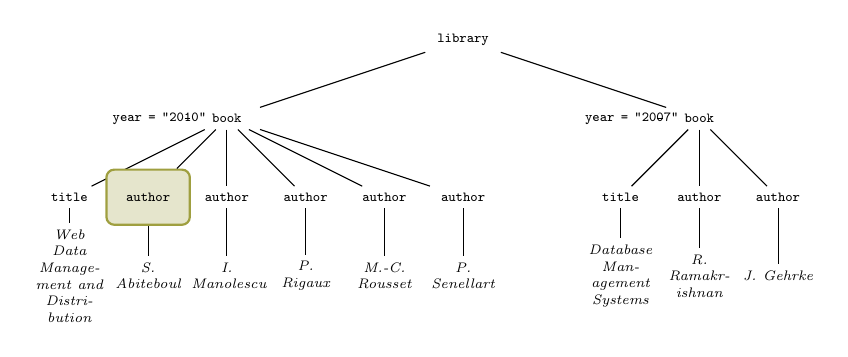
\begin{tikzpicture}[auto]
\tiny
  \tikzstyle{emptyStyle}=[text width=0.9cm, text centered]
  \tikzstyle{red}=[rounded corners=1mm,thick,draw=red!75,fill=red!20,text width=0.9cm, text centered]
  \tikzstyle{DarkViolet}=[rounded corners=1mm,thick,draw=DarkViolet!75,fill=DarkViolet!20,minimum size=7mm,text width=0.8cm, text centered]
  \tikzstyle{green}=[rounded corners=1mm,thick,draw=DarkOliveGreen!75,fill=DarkOliveGreen!20,minimum size=7mm,text width=0.8cm, text centered]
  \tikzstyle{cyan}=[rounded corners=1mm,thick,draw=DarkCyan!75,fill=DarkCyan!20,minimum size=7mm,text width=0.8cm, text centered]
 \tikzstyle{every label}=[black]
  \tikzstyle{HotPink}=[rounded corners=1mm,thick,draw=HotPink!75,fill=HotPink!20,minimum size=7mm,text width=0.8cm, text centered]
  \tikzstyle{noeudcourant}=[rounded corners=1mm,thick,draw=Olive!75,fill=Olive!20,minimum size=7mm,text width=0.9cm, text centered]
  \tikzstyle{indiaRed}=[rounded corners=1mm,thick,draw=indiaRed!75,fill=indiaRed!20,minimum size=7mm,text width=0.9cm, text centered]

  \begin{scope}
   % \node[emptyStyle](r) at (7,5) {Root};  
   %\node[emptyStyle](entete) at (3,4) {\texttt{$<?xml$ version $...>$}};
   %\draw[-] (r) -- (entete);
   \node[emptyStyle](library) at (7,4) {\verb?library?};
   % \draw[-] (r) -- (library);

    \node[emptyStyle](book1) at (4,3) {\verb?book?};
   \draw[-] (library) -- (book1);
   \node[emptyStyle](book2) at (10,3) {\verb?book?};
   \draw[-] (library) -- (book2);

    \node[emptyStyle](year1) at (3,3) {\verb?year = "2010"?};
   \draw[-] (book1) -- (year1);
    \node[emptyStyle](title1) at (2,2) {\verb?title?};
   \draw[-] (book1) -- (title1);
 \node[emptyStyle](texttitle1) at (2,1) {\it Web Data Management and Distribution};
   \draw[-] (title1) -- (texttitle1);
    \node[noeudcourant](author1) at (3,2) {\verb?author?};
   \draw[-] (book1) -- (author1);
   \node[emptyStyle](textauthor1) at (3,1) {\it S. Abiteboul};
   \draw[-] (author1) -- (textauthor1);
    \node[emptyStyle](author2) at (4,2) {\verb?author?};
   \draw[-] (book1) -- (author2);
   \node[emptyStyle](textauthor2) at (4,1) {\it I. Manolescu};
   \draw[-] (author2) -- (textauthor2);
    \node[emptyStyle](author3) at (5,2) {\verb?author?};
   \draw[-] (book1) -- (author3);
   \node[emptyStyle](textauthor3) at (5,1) {\it P. Rigaux};
   \draw[-] (author3) -- (textauthor3);
    \node[emptyStyle](author4) at (6,2) {\verb?author?};
   \draw[-] (book1) -- (author4);
   \node[emptyStyle](textauthor4) at (6,1) {\it M.-C. Rousset};
   \draw[-] (author4) -- (textauthor4);
    \node[emptyStyle](author5) at (7,2) {\verb?author?};
   \draw[-] (book1) -- (author5);
   \node[emptyStyle](textauthor5) at (7,1) {\it P. Senellart};
   \draw[-] (author5) -- (textauthor5);

    \node[emptyStyle](year2) at (9,3) {\verb?year = "2007"?};
   \draw[-] (book2) -- (year2);
    \node[emptyStyle](title2) at (9,2) {\verb?title?};
   \draw[-] (book2) -- (title2);
 \node[emptyStyle](texttitle2) at (9,1) {\it Database Management Systems};
   \draw[-] (title2) -- (texttitle2);
    \node[emptyStyle](author1prime) at (10,2) {\verb?author?};
   \draw[-] (book2) -- (author1prime);
   \node[emptyStyle](textauthor1prime) at (10,1) {\it R. Ramakrishnan};
   \draw[-] (author1prime) -- (textauthor1prime);
    \node[emptyStyle](author2prime) at (11,2) {\verb?author?};
   \draw[-] (book2) -- (author2prime);
   \node[emptyStyle](textauthor2prime) at (11,1) {\it J. Gehrke};
   \draw[-] (author2prime) -- (textauthor2prime);
\end{scope}
\end{tikzpicture}
\end{frame}


\begin{frame}{Quelques axes en exemple : \texttt{parent}}
\texttt{parent} : le parent du n{\oe}ud courant.

\bigskip

\begin{tikzpicture}[auto]
\tiny
  \tikzstyle{emptyStyle}=[text width=0.9cm, text centered]
  \tikzstyle{red}=[rounded corners=1mm,thick,draw=red!75,fill=red!20,text width=0.9cm, text centered]
  \tikzstyle{DarkViolet}=[rounded corners=1mm,thick,draw=DarkViolet!75,fill=DarkViolet!20,minimum size=7mm,text width=0.8cm, text centered]
  \tikzstyle{green}=[rounded corners=1mm,thick,draw=DarkOliveGreen!75,fill=DarkOliveGreen!20,minimum size=7mm,text width=0.8cm, text centered]
  \tikzstyle{cyan}=[rounded corners=1mm,thick,draw=DarkCyan!75,fill=DarkCyan!20,minimum size=7mm,text width=0.8cm, text centered]
 \tikzstyle{every label}=[black]
  \tikzstyle{HotPink}=[rounded corners=1mm,thick,draw=HotPink!75,fill=HotPink!20,minimum size=7mm,text width=0.8cm, text centered]
  \tikzstyle{noeudcourant}=[rounded corners=1mm,thick,draw=Olive!75,fill=Olive!20,minimum size=7mm,text width=0.9cm, text centered]
  \tikzstyle{indiaRed}=[rounded corners=1mm,thick,draw=indiaRed!75,fill=indiaRed!20,minimum size=7mm,text width=0.9cm, text centered]

  \begin{scope}
   % \node[emptyStyle](r) at (7,5) {Root};  
   %\node[emptyStyle](entete) at (3,4) {\texttt{$<?xml$ version $...>$}};
   %\draw[-] (r) -- (entete);
   \node[emptyStyle](library) at (7,4) {\verb?library?};
   % \draw[-] (r) -- (library);

    \node[indiaRed](book1) at (4,3) {\verb?book?};
   \draw[-] (library) -- (book1);
   \node[emptyStyle](book2) at (10,3) {\verb?book?};
   \draw[-] (library) -- (book2);

    \node[emptyStyle](year1) at (3,3) {\verb?year = "2010"?};
   \draw[-] (book1) -- (year1);
    \node[emptyStyle](title1) at (2,2) {\verb?title?};
   \draw[-] (book1) -- (title1);
 \node[emptyStyle](texttitle1) at (2,1) {\it Web Data Management and Distribution};
   \draw[-] (title1) -- (texttitle1);
    \node[noeudcourant](author1) at (3,2) {\verb?author?};
   \draw[-] (book1) -- (author1);
   \node[emptyStyle](textauthor1) at (3,1) {\it S. Abiteboul};
   \draw[-] (author1) -- (textauthor1);
    \node[emptyStyle](author2) at (4,2) {\verb?author?};
   \draw[-] (book1) -- (author2);
   \node[emptyStyle](textauthor2) at (4,1) {\it I. Manolescu};
   \draw[-] (author2) -- (textauthor2);
    \node[emptyStyle](author3) at (5,2) {\verb?author?};
   \draw[-] (book1) -- (author3);
   \node[emptyStyle](textauthor3) at (5,1) {\it P. Rigaux};
   \draw[-] (author3) -- (textauthor3);
    \node[emptyStyle](author4) at (6,2) {\verb?author?};
   \draw[-] (book1) -- (author4);
   \node[emptyStyle](textauthor4) at (6,1) {\it M.-C. Rousset};
   \draw[-] (author4) -- (textauthor4);
    \node[emptyStyle](author5) at (7,2) {\verb?author?};
   \draw[-] (book1) -- (author5);
   \node[emptyStyle](textauthor5) at (7,1) {\it P. Senellart};
   \draw[-] (author5) -- (textauthor5);

    \node[emptyStyle](year2) at (9,3) {\verb?year = "2007"?};
   \draw[-] (book2) -- (year2);
    \node[emptyStyle](title2) at (9,2) {\verb?title?};
   \draw[-] (book2) -- (title2);
 \node[emptyStyle](texttitle2) at (9,1) {\it Database Management Systems};
   \draw[-] (title2) -- (texttitle2);
    \node[emptyStyle](author1prime) at (10,2) {\verb?author?};
   \draw[-] (book2) -- (author1prime);
   \node[emptyStyle](textauthor1prime) at (10,1) {\it R. Ramakrishnan};
   \draw[-] (author1prime) -- (textauthor1prime);
    \node[emptyStyle](author2prime) at (11,2) {\verb?author?};
   \draw[-] (book2) -- (author2prime);
   \node[emptyStyle](textauthor2prime) at (11,1) {\it J. Gehrke};
   \draw[-] (author2prime) -- (textauthor2prime);
\end{scope}
\end{tikzpicture}
\end{frame}

\begin{frame}{Quelques axes en exemple : \texttt{parent}}
\texttt{parent} : le parent du n{\oe}ud courant.

\bigskip

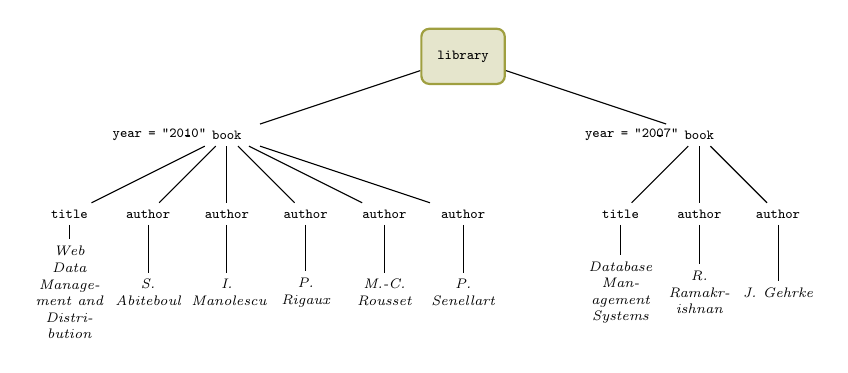
\begin{tikzpicture}[auto]
\tiny
  \tikzstyle{emptyStyle}=[text width=0.9cm, text centered]
  \tikzstyle{red}=[rounded corners=1mm,thick,draw=red!75,fill=red!20,text width=0.9cm, text centered]
  \tikzstyle{DarkViolet}=[rounded corners=1mm,thick,draw=DarkViolet!75,fill=DarkViolet!20,minimum size=7mm,text width=0.8cm, text centered]
  \tikzstyle{green}=[rounded corners=1mm,thick,draw=DarkOliveGreen!75,fill=DarkOliveGreen!20,minimum size=7mm,text width=0.8cm, text centered]
  \tikzstyle{cyan}=[rounded corners=1mm,thick,draw=DarkCyan!75,fill=DarkCyan!20,minimum size=7mm,text width=0.8cm, text centered]
 \tikzstyle{every label}=[black]
  \tikzstyle{HotPink}=[rounded corners=1mm,thick,draw=HotPink!75,fill=HotPink!20,minimum size=7mm,text width=0.8cm, text centered]
  \tikzstyle{noeudcourant}=[rounded corners=1mm,thick,draw=Olive!75,fill=Olive!20,minimum size=7mm,text width=0.9cm, text centered]
  \tikzstyle{indiaRed}=[rounded corners=1mm,thick,draw=indiaRed!75,fill=indiaRed!20,minimum size=7mm,text width=0.9cm, text centered]

  \begin{scope}
   % \node[emptyStyle](r) at (7,5) {Root};  
   %\node[emptyStyle](entete) at (3,4) {\texttt{$<?xml$ version $...>$}};
   %\draw[-] (r) -- (entete);
   \node[noeudcourant](library) at (7,4) {\verb?library?};
   % \draw[-] (r) -- (library);

    \node[emptyStyle](book1) at (4,3) {\verb?book?};
   \draw[-] (library) -- (book1);
   \node[emptyStyle](book2) at (10,3) {\verb?book?};
   \draw[-] (library) -- (book2);

    \node[emptyStyle](year1) at (3,3) {\verb?year = "2010"?};
   \draw[-] (book1) -- (year1);
    \node[emptyStyle](title1) at (2,2) {\verb?title?};
   \draw[-] (book1) -- (title1);
 \node[emptyStyle](texttitle1) at (2,1) {\it Web Data Management and Distribution};
   \draw[-] (title1) -- (texttitle1);
    \node[emptyStyle](author1) at (3,2) {\verb?author?};
   \draw[-] (book1) -- (author1);
   \node[emptyStyle](textauthor1) at (3,1) {\it S. Abiteboul};
   \draw[-] (author1) -- (textauthor1);
    \node[emptyStyle](author2) at (4,2) {\verb?author?};
   \draw[-] (book1) -- (author2);
   \node[emptyStyle](textauthor2) at (4,1) {\it I. Manolescu};
   \draw[-] (author2) -- (textauthor2);
    \node[emptyStyle](author3) at (5,2) {\verb?author?};
   \draw[-] (book1) -- (author3);
   \node[emptyStyle](textauthor3) at (5,1) {\it P. Rigaux};
   \draw[-] (author3) -- (textauthor3);
    \node[emptyStyle](author4) at (6,2) {\verb?author?};
   \draw[-] (book1) -- (author4);
   \node[emptyStyle](textauthor4) at (6,1) {\it M.-C. Rousset};
   \draw[-] (author4) -- (textauthor4);
    \node[emptyStyle](author5) at (7,2) {\verb?author?};
   \draw[-] (book1) -- (author5);
   \node[emptyStyle](textauthor5) at (7,1) {\it P. Senellart};
   \draw[-] (author5) -- (textauthor5);

    \node[emptyStyle](year2) at (9,3) {\verb?year = "2007"?};
   \draw[-] (book2) -- (year2);
    \node[emptyStyle](title2) at (9,2) {\verb?title?};
   \draw[-] (book2) -- (title2);
 \node[emptyStyle](texttitle2) at (9,1) {\it Database Management Systems};
   \draw[-] (title2) -- (texttitle2);
    \node[emptyStyle](author1prime) at (10,2) {\verb?author?};
   \draw[-] (book2) -- (author1prime);
   \node[emptyStyle](textauthor1prime) at (10,1) {\it R. Ramakrishnan};
   \draw[-] (author1prime) -- (textauthor1prime);
    \node[emptyStyle](author2prime) at (11,2) {\verb?author?};
   \draw[-] (book2) -- (author2prime);
   \node[emptyStyle](textauthor2prime) at (11,1) {\it J. Gehrke};
   \draw[-] (author2prime) -- (textauthor2prime);
\end{scope}
\end{tikzpicture}
\prof{Pas de n{\oe}ud parent}

\end{frame}


% ancestor
\subsection{Ancestor}

\begin{frame}{Quelques axes en exemple : \texttt{ancestor}}
\texttt{ancestor} : tous les ancêtres  (parent, grand-parent, etc.) du n{\oe}ud courant.

\bigskip

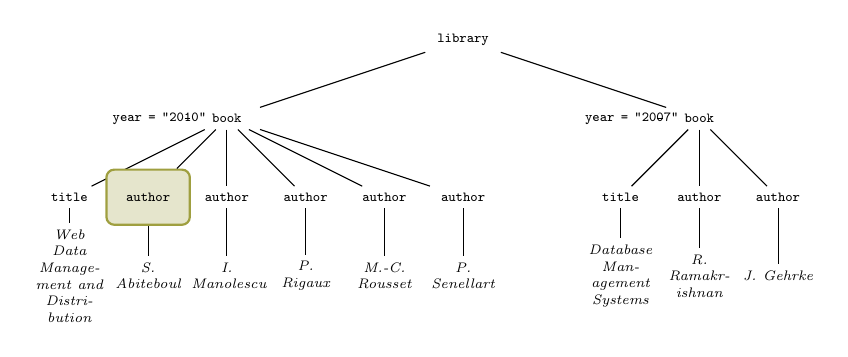
\begin{tikzpicture}[auto]
\tiny
  \tikzstyle{emptyStyle}=[text width=0.9cm, text centered]
  \tikzstyle{red}=[rounded corners=1mm,thick,draw=red!75,fill=red!20,text width=0.9cm, text centered]
  \tikzstyle{DarkViolet}=[rounded corners=1mm,thick,draw=DarkViolet!75,fill=DarkViolet!20,minimum size=7mm,text width=0.8cm, text centered]
  \tikzstyle{green}=[rounded corners=1mm,thick,draw=DarkOliveGreen!75,fill=DarkOliveGreen!20,minimum size=7mm,text width=0.8cm, text centered]
  \tikzstyle{cyan}=[rounded corners=1mm,thick,draw=DarkCyan!75,fill=DarkCyan!20,minimum size=7mm,text width=0.8cm, text centered]
 \tikzstyle{every label}=[black]
  \tikzstyle{HotPink}=[rounded corners=1mm,thick,draw=HotPink!75,fill=HotPink!20,minimum size=7mm,text width=0.8cm, text centered]
  \tikzstyle{noeudcourant}=[rounded corners=1mm,thick,draw=Olive!75,fill=Olive!20,minimum size=7mm,text width=0.9cm, text centered]
  \tikzstyle{indiaRed}=[rounded corners=1mm,thick,draw=indiaRed!75,fill=indiaRed!20,minimum size=7mm,text width=0.9cm, text centered]

  \begin{scope}
   % \node[emptyStyle](r) at (7,5) {Root};  
   %\node[emptyStyle](entete) at (3,4) {\texttt{$<?xml$ version $...>$}};
   %\draw[-] (r) -- (entete);
   \node[emptyStyle](library) at (7,4) {\verb?library?};
   % \draw[-] (r) -- (library);

    \node[emptyStyle](book1) at (4,3) {\verb?book?};
   \draw[-] (library) -- (book1);
   \node[emptyStyle](book2) at (10,3) {\verb?book?};
   \draw[-] (library) -- (book2);

    \node[emptyStyle](year1) at (3,3) {\verb?year = "2010"?};
   \draw[-] (book1) -- (year1);
    \node[emptyStyle](title1) at (2,2) {\verb?title?};
   \draw[-] (book1) -- (title1);
 \node[emptyStyle](texttitle1) at (2,1) {\it Web Data Management and Distribution};
   \draw[-] (title1) -- (texttitle1);
    \node[noeudcourant](author1) at (3,2) {\verb?author?};
   \draw[-] (book1) -- (author1);
   \node[emptyStyle](textauthor1) at (3,1) {\it S. Abiteboul};
   \draw[-] (author1) -- (textauthor1);
    \node[emptyStyle](author2) at (4,2) {\verb?author?};
   \draw[-] (book1) -- (author2);
   \node[emptyStyle](textauthor2) at (4,1) {\it I. Manolescu};
   \draw[-] (author2) -- (textauthor2);
    \node[emptyStyle](author3) at (5,2) {\verb?author?};
   \draw[-] (book1) -- (author3);
   \node[emptyStyle](textauthor3) at (5,1) {\it P. Rigaux};
   \draw[-] (author3) -- (textauthor3);
    \node[emptyStyle](author4) at (6,2) {\verb?author?};
   \draw[-] (book1) -- (author4);
   \node[emptyStyle](textauthor4) at (6,1) {\it M.-C. Rousset};
   \draw[-] (author4) -- (textauthor4);
    \node[emptyStyle](author5) at (7,2) {\verb?author?};
   \draw[-] (book1) -- (author5);
   \node[emptyStyle](textauthor5) at (7,1) {\it P. Senellart};
   \draw[-] (author5) -- (textauthor5);

    \node[emptyStyle](year2) at (9,3) {\verb?year = "2007"?};
   \draw[-] (book2) -- (year2);
    \node[emptyStyle](title2) at (9,2) {\verb?title?};
   \draw[-] (book2) -- (title2);
 \node[emptyStyle](texttitle2) at (9,1) {\it Database Management Systems};
   \draw[-] (title2) -- (texttitle2);
    \node[emptyStyle](author1prime) at (10,2) {\verb?author?};
   \draw[-] (book2) -- (author1prime);
   \node[emptyStyle](textauthor1prime) at (10,1) {\it R. Ramakrishnan};
   \draw[-] (author1prime) -- (textauthor1prime);
    \node[emptyStyle](author2prime) at (11,2) {\verb?author?};
   \draw[-] (book2) -- (author2prime);
   \node[emptyStyle](textauthor2prime) at (11,1) {\it J. Gehrke};
   \draw[-] (author2prime) -- (textauthor2prime);
\end{scope}
\end{tikzpicture}
\end{frame}


 \begin{frame}{Quelques axes en exemple : \texttt{ancestor}}
\texttt{ancestor} : tous les ancêtres  (parent, grand-parent, etc.) du n{\oe}ud courant.

\bigskip

\begin{tikzpicture}[auto]
\tiny
  \tikzstyle{emptyStyle}=[text width=0.9cm, text centered]
  \tikzstyle{red}=[rounded corners=1mm,thick,draw=red!75,fill=red!20,text width=0.9cm, text centered]
  \tikzstyle{DarkViolet}=[rounded corners=1mm,thick,draw=DarkViolet!75,fill=DarkViolet!20,minimum size=7mm,text width=0.8cm, text centered]
  \tikzstyle{green}=[rounded corners=1mm,thick,draw=DarkOliveGreen!75,fill=DarkOliveGreen!20,minimum size=7mm,text width=0.8cm, text centered]
  \tikzstyle{cyan}=[rounded corners=1mm,thick,draw=DarkCyan!75,fill=DarkCyan!20,minimum size=7mm,text width=0.8cm, text centered]
 \tikzstyle{every label}=[black]
  \tikzstyle{HotPink}=[rounded corners=1mm,thick,draw=HotPink!75,fill=HotPink!20,minimum size=7mm,text width=0.8cm, text centered]
  \tikzstyle{noeudcourant}=[rounded corners=1mm,thick,draw=Olive!75,fill=Olive!20,minimum size=7mm,text width=0.9cm, text centered]
  \tikzstyle{indiaRed}=[rounded corners=1mm,thick,draw=indiaRed!75,fill=indiaRed!20,minimum size=7mm,text width=0.9cm, text centered]

  \begin{scope}
   % \node[emptyStyle](r) at (7,5) {Root};  
   %\node[emptyStyle](entete) at (3,4) {\texttt{$<?xml$ version $...>$}};
   %\draw[-] (r) -- (entete);
   \node[indiaRed](library) at (7,4) {\verb?library?};
   % \draw[-] (r) -- (library);

    \node[indiaRed](book1) at (4,3) {\verb?book?};
   \draw[-] (library) -- (book1);
   \node[emptyStyle](book2) at (10,3) {\verb?book?};
   \draw[-] (library) -- (book2);

    \node[emptyStyle](year1) at (3,3) {\verb?year = "2010"?};
   \draw[-] (book1) -- (year1);
    \node[emptyStyle](title1) at (2,2) {\verb?title?};
   \draw[-] (book1) -- (title1);
 \node[emptyStyle](texttitle1) at (2,1) {\it Web Data Management and Distribution};
   \draw[-] (title1) -- (texttitle1);
    \node[noeudcourant](author1) at (3,2) {\verb?author?};
   \draw[-] (book1) -- (author1);
   \node[emptyStyle](textauthor1) at (3,1) {\it S. Abiteboul};
   \draw[-] (author1) -- (textauthor1);
    \node[emptyStyle](author2) at (4,2) {\verb?author?};
   \draw[-] (book1) -- (author2);
   \node[emptyStyle](textauthor2) at (4,1) {\it I. Manolescu};
   \draw[-] (author2) -- (textauthor2);
    \node[emptyStyle](author3) at (5,2) {\verb?author?};
   \draw[-] (book1) -- (author3);
   \node[emptyStyle](textauthor3) at (5,1) {\it P. Rigaux};
   \draw[-] (author3) -- (textauthor3);
    \node[emptyStyle](author4) at (6,2) {\verb?author?};
   \draw[-] (book1) -- (author4);
   \node[emptyStyle](textauthor4) at (6,1) {\it M.-C. Rousset};
   \draw[-] (author4) -- (textauthor4);
    \node[emptyStyle](author5) at (7,2) {\verb?author?};
   \draw[-] (book1) -- (author5);
   \node[emptyStyle](textauthor5) at (7,1) {\it P. Senellart};
   \draw[-] (author5) -- (textauthor5);

    \node[emptyStyle](year2) at (9,3) {\verb?year = "2007"?};
   \draw[-] (book2) -- (year2);
    \node[emptyStyle](title2) at (9,2) {\verb?title?};
   \draw[-] (book2) -- (title2);
 \node[emptyStyle](texttitle2) at (9,1) {\it Database Management Systems};
   \draw[-] (title2) -- (texttitle2);
    \node[emptyStyle](author1prime) at (10,2) {\verb?author?};
   \draw[-] (book2) -- (author1prime);
   \node[emptyStyle](textauthor1prime) at (10,1) {\it R. Ramakrishnan};
   \draw[-] (author1prime) -- (textauthor1prime);
    \node[emptyStyle](author2prime) at (11,2) {\verb?author?};
   \draw[-] (book2) -- (author2prime);
   \node[emptyStyle](textauthor2prime) at (11,1) {\it J. Gehrke};
   \draw[-] (author2prime) -- (textauthor2prime);
\end{scope}
\end{tikzpicture}
\end{frame}

\subsection{Ancestor-or-self}

 \begin{frame}{Quelques axes en exemple :\texttt{ancestor-or-self}}
\texttt{ancestor-or-self} : tous les ancêtres  (parent, grand-parent, etc.) du n{\oe}ud courant \alert{et} le n{\oe}ud courant
lui-même.

\bigskip

\begin{tikzpicture}[auto]
\tiny
  \tikzstyle{emptyStyle}=[text width=0.9cm, text centered]
  \tikzstyle{red}=[rounded corners=1mm,thick,draw=red!75,fill=red!20,text width=0.9cm, text centered]
  \tikzstyle{DarkViolet}=[rounded corners=1mm,thick,draw=DarkViolet!75,fill=DarkViolet!20,minimum size=7mm,text width=0.8cm, text centered]
  \tikzstyle{green}=[rounded corners=1mm,thick,draw=DarkOliveGreen!75,fill=DarkOliveGreen!20,minimum size=7mm,text width=0.8cm, text centered]
  \tikzstyle{cyan}=[rounded corners=1mm,thick,draw=DarkCyan!75,fill=DarkCyan!20,minimum size=7mm,text width=0.8cm, text centered]
 \tikzstyle{every label}=[black]
  \tikzstyle{HotPink}=[rounded corners=1mm,thick,draw=HotPink!75,fill=HotPink!20,minimum size=7mm,text width=0.8cm, text centered]
  \tikzstyle{noeudcourant}=[rounded corners=1mm,thick,draw=Olive!75,fill=Olive!20,minimum size=7mm,text width=0.9cm, text centered]
  \tikzstyle{indiaRed}=[rounded corners=1mm,thick,draw=indiaRed!75,fill=indiaRed!20,minimum size=7mm,text width=0.9cm, text centered]

  \begin{scope}
   % \node[emptyStyle](r) at (7,5) {Root};  
   %\node[emptyStyle](entete) at (3,4) {\texttt{$<?xml$ version $...>$}};
   %\draw[-] (r) -- (entete);
   \node[indiaRed](library) at (7,4) {\verb?library?};
   % \draw[-] (r) -- (library);

    \node[indiaRed](book1) at (4,3) {\verb?book?};
   \draw[-] (library) -- (book1);
   \node[emptyStyle](book2) at (10,3) {\verb?book?};
   \draw[-] (library) -- (book2);

    \node[emptyStyle](year1) at (3,3) {\verb?year = "2010"?};
   \draw[-] (book1) -- (year1);
    \node[emptyStyle](title1) at (2,2) {\verb?title?};
   \draw[-] (book1) -- (title1);
 \node[emptyStyle](texttitle1) at (2,1) {\it Web Data Management and Distribution};
   \draw[-] (title1) -- (texttitle1);
    \node[indiaRed](author1) at (3,2) {\verb?author?};
   \draw[-] (book1) -- (author1);
   \node[emptyStyle](textauthor1) at (3,1) {\it S. Abiteboul};
   \draw[-] (author1) -- (textauthor1);
    \node[emptyStyle](author2) at (4,2) {\verb?author?};
   \draw[-] (book1) -- (author2);
   \node[emptyStyle](textauthor2) at (4,1) {\it I. Manolescu};
   \draw[-] (author2) -- (textauthor2);
    \node[emptyStyle](author3) at (5,2) {\verb?author?};
   \draw[-] (book1) -- (author3);
   \node[emptyStyle](textauthor3) at (5,1) {\it P. Rigaux};
   \draw[-] (author3) -- (textauthor3);
    \node[emptyStyle](author4) at (6,2) {\verb?author?};
   \draw[-] (book1) -- (author4);
   \node[emptyStyle](textauthor4) at (6,1) {\it M.-C. Rousset};
   \draw[-] (author4) -- (textauthor4);
    \node[emptyStyle](author5) at (7,2) {\verb?author?};
   \draw[-] (book1) -- (author5);
   \node[emptyStyle](textauthor5) at (7,1) {\it P. Senellart};
   \draw[-] (author5) -- (textauthor5);

    \node[emptyStyle](year2) at (9,3) {\verb?year = "2007"?};
   \draw[-] (book2) -- (year2);
    \node[emptyStyle](title2) at (9,2) {\verb?title?};
   \draw[-] (book2) -- (title2);
 \node[emptyStyle](texttitle2) at (9,1) {\it Database Management Systems};
   \draw[-] (title2) -- (texttitle2);
    \node[emptyStyle](author1prime) at (10,2) {\verb?author?};
   \draw[-] (book2) -- (author1prime);
   \node[emptyStyle](textauthor1prime) at (10,1) {\it R. Ramakrishnan};
   \draw[-] (author1prime) -- (textauthor1prime);
    \node[emptyStyle](author2prime) at (11,2) {\verb?author?};
   \draw[-] (book2) -- (author2prime);
   \node[emptyStyle](textauthor2prime) at (11,1) {\it J. Gehrke};
   \draw[-] (author2prime) -- (textauthor2prime);
\end{scope}
\end{tikzpicture}


\prof{Exercice : ancestor et ancestor-or-self sur la biblio (racine)}
\end{frame}



\subsection{Descendant}
% descendant

\begin{frame}{Quelques axes en exemple : \texttt{descendant}}
\texttt{descendant} : tous les  descendants (enfants, petits-enfants, ) du n{\oe}ud courant.

\bigskip

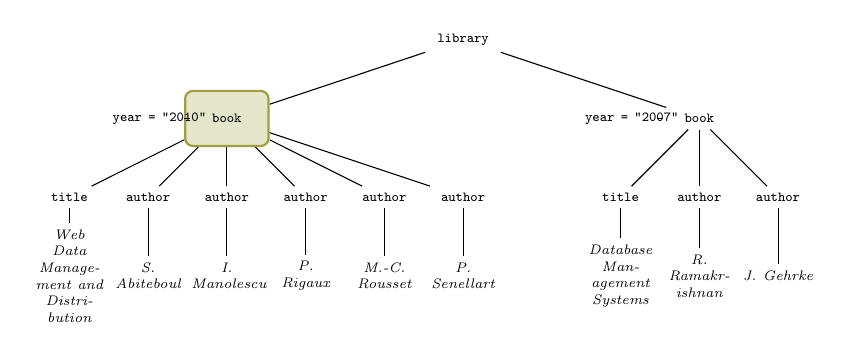
\begin{tikzpicture}[auto]
\tiny
  \tikzstyle{emptyStyle}=[text width=0.9cm, text centered]
  \tikzstyle{red}=[rounded corners=1mm,thick,draw=red!75,fill=red!20,text width=0.9cm, text centered]
  \tikzstyle{DarkViolet}=[rounded corners=1mm,thick,draw=DarkViolet!75,fill=DarkViolet!20,minimum size=7mm,text width=0.8cm, text centered]
  \tikzstyle{green}=[rounded corners=1mm,thick,draw=DarkOliveGreen!75,fill=DarkOliveGreen!20,minimum size=7mm,text width=0.8cm, text centered]
  \tikzstyle{cyan}=[rounded corners=1mm,thick,draw=DarkCyan!75,fill=DarkCyan!20,minimum size=7mm,text width=0.8cm, text centered]
 \tikzstyle{every label}=[black]
  \tikzstyle{HotPink}=[rounded corners=1mm,thick,draw=HotPink!75,fill=HotPink!20,minimum size=7mm,text width=0.8cm, text centered]
  \tikzstyle{noeudcourant}=[rounded corners=1mm,thick,draw=Olive!75,fill=Olive!20,minimum size=7mm,text width=0.9cm, text centered]
  \tikzstyle{indiaRed}=[rounded corners=1mm,thick,draw=indiaRed!75,fill=indiaRed!20,minimum size=7mm,text width=0.9cm, text centered]

  \begin{scope}
   % \node[emptyStyle](r) at (7,5) {Root};  
   %\node[emptyStyle](entete) at (3,4) {\texttt{$<?xml$ version $...>$}};
   %\draw[-] (r) -- (entete);
   \node[emptyStyle](library) at (7,4) {\verb?library?};
   % \draw[-] (r) -- (library);

    \node[noeudcourant](book1) at (4,3) {\verb?book?};
   \draw[-] (library) -- (book1);
   \node[emptyStyle](book2) at (10,3) {\verb?book?};
   \draw[-] (library) -- (book2);

    \node[emptyStyle](year1) at (3,3) {\verb?year = "2010"?};
   \draw[-] (book1) -- (year1);
    \node[emptyStyle](title1) at (2,2) {\verb?title?};
   \draw[-] (book1) -- (title1);
 \node[emptyStyle](texttitle1) at (2,1) {\it Web Data Management and Distribution};
   \draw[-] (title1) -- (texttitle1);
    \node[emptyStyle](author1) at (3,2) {\verb?author?};
   \draw[-] (book1) -- (author1);
   \node[emptyStyle](textauthor1) at (3,1) {\it S. Abiteboul};
   \draw[-] (author1) -- (textauthor1);
    \node[emptyStyle](author2) at (4,2) {\verb?author?};
   \draw[-] (book1) -- (author2);
   \node[emptyStyle](textauthor2) at (4,1) {\it I. Manolescu};
   \draw[-] (author2) -- (textauthor2);
    \node[emptyStyle](author3) at (5,2) {\verb?author?};
   \draw[-] (book1) -- (author3);
   \node[emptyStyle](textauthor3) at (5,1) {\it P. Rigaux};
   \draw[-] (author3) -- (textauthor3);
    \node[emptyStyle](author4) at (6,2) {\verb?author?};
   \draw[-] (book1) -- (author4);
   \node[emptyStyle](textauthor4) at (6,1) {\it M.-C. Rousset};
   \draw[-] (author4) -- (textauthor4);
    \node[emptyStyle](author5) at (7,2) {\verb?author?};
   \draw[-] (book1) -- (author5);
   \node[emptyStyle](textauthor5) at (7,1) {\it P. Senellart};
   \draw[-] (author5) -- (textauthor5);

    \node[emptyStyle](year2) at (9,3) {\verb?year = "2007"?};
   \draw[-] (book2) -- (year2);
    \node[emptyStyle](title2) at (9,2) {\verb?title?};
   \draw[-] (book2) -- (title2);
 \node[emptyStyle](texttitle2) at (9,1) {\it Database Management Systems};
   \draw[-] (title2) -- (texttitle2);
    \node[emptyStyle](author1prime) at (10,2) {\verb?author?};
   \draw[-] (book2) -- (author1prime);
   \node[emptyStyle](textauthor1prime) at (10,1) {\it R. Ramakrishnan};
   \draw[-] (author1prime) -- (textauthor1prime);
    \node[emptyStyle](author2prime) at (11,2) {\verb?author?};
   \draw[-] (book2) -- (author2prime);
   \node[emptyStyle](textauthor2prime) at (11,1) {\it J. Gehrke};
   \draw[-] (author2prime) -- (textauthor2prime);
\end{scope}
\end{tikzpicture}
\end{frame}


 \begin{frame}{Quelques axes en exemple : \texttt{descendant}}
\texttt{descendant} : tous les  descendants (enfants, petits-enfants, ) du n{\oe}ud courant.

\bigskip

\begin{tikzpicture}[auto]
\tiny
  \tikzstyle{emptyStyle}=[text width=0.9cm, text centered]
  \tikzstyle{red}=[rounded corners=1mm,thick,draw=red!75,fill=red!20,text width=0.9cm, text centered]
  \tikzstyle{DarkViolet}=[rounded corners=1mm,thick,draw=DarkViolet!75,fill=DarkViolet!20,minimum size=7mm,text width=0.8cm, text centered]
  \tikzstyle{green}=[rounded corners=1mm,thick,draw=DarkOliveGreen!75,fill=DarkOliveGreen!20,minimum size=7mm,text width=0.8cm, text centered]
  \tikzstyle{cyan}=[rounded corners=1mm,thick,draw=DarkCyan!75,fill=DarkCyan!20,minimum size=7mm,text width=0.8cm, text centered]
 \tikzstyle{every label}=[black]
  \tikzstyle{HotPink}=[rounded corners=1mm,thick,draw=HotPink!75,fill=HotPink!20,minimum size=7mm,text width=0.8cm, text centered]
  \tikzstyle{noeudcourant}=[rounded corners=1mm,thick,draw=Olive!75,fill=Olive!20,minimum size=7mm,text width=0.9cm, text centered]
  \tikzstyle{indiaRed}=[rounded corners=1mm,thick,draw=indiaRed!75,fill=indiaRed!20,minimum size=7mm,text width=0.9cm, text centered]

  \begin{scope}
   % \node[emptyStyle](r) at (7,5) {Root};  
   %\node[emptyStyle](entete) at (3,4) {\texttt{$<?xml$ version $...>$}};
   %\draw[-] (r) -- (entete);
   \node[emptyStyle](library) at (7,4) {\verb?library?};
   % \draw[-] (r) -- (library);

    \node[noeudcourant](book1) at (4,3) {\verb?book?};
   \draw[-] (library) -- (book1);
   \node[emptyStyle](book2) at (10,3) {\verb?book?};
   \draw[-] (library) -- (book2);

    \node[emptyStyle](year1) at (3,3) {\verb?year = "2010"?};
   \draw[-] (book1) -- (year1);
    \node[indiaRed](title1) at (2,2) {\verb?title?};
   \draw[-] (book1) -- (title1);
 \node[indiaRed](texttitle1) at (2,1) {\it Web Data Management and Distribution};
   \draw[-] (title1) -- (texttitle1);
    \node[indiaRed](author1) at (3,2) {\verb?author?};
   \draw[-] (book1) -- (author1);
   \node[indiaRed](textauthor1) at (3,1) {\it S. Abiteboul};
   \draw[-] (author1) -- (textauthor1);
    \node[indiaRed](author2) at (4,2) {\verb?author?};
   \draw[-] (book1) -- (author2);
   \node[indiaRed](textauthor2) at (4,1) {\it I. Manolescu};
   \draw[-] (author2) -- (textauthor2);
    \node[indiaRed](author3) at (5,2) {\verb?author?};
   \draw[-] (book1) -- (author3);
   \node[indiaRed](textauthor3) at (5,1) {\it P. Rigaux};
   \draw[-] (author3) -- (textauthor3);
    \node[indiaRed](author4) at (6,2) {\verb?author?};
   \draw[-] (book1) -- (author4);
   \node[indiaRed](textauthor4) at (6,1) {\it M.-C. Rousset};
   \draw[-] (author4) -- (textauthor4);
    \node[indiaRed](author5) at (7,2) {\verb?author?};
   \draw[-] (book1) -- (author5);
   \node[indiaRed](textauthor5) at (7,1) {\it P. Senellart};
   \draw[-] (author5) -- (textauthor5);

    \node[emptyStyle](year2) at (9,3) {\verb?year = "2007"?};
   \draw[-] (book2) -- (year2);
    \node[emptyStyle](title2) at (9,2) {\verb?title?};
   \draw[-] (book2) -- (title2);
 \node[emptyStyle](texttitle2) at (9,1) {\it Database Management Systems};
   \draw[-] (title2) -- (texttitle2);
    \node[emptyStyle](author1prime) at (10,2) {\verb?author?};
   \draw[-] (book2) -- (author1prime);
   \node[emptyStyle](textauthor1prime) at (10,1) {\it R. Ramakrishnan};
   \draw[-] (author1prime) -- (textauthor1prime);
    \node[emptyStyle](author2prime) at (11,2) {\verb?author?};
   \draw[-] (book2) -- (author2prime);
   \node[emptyStyle](textauthor2prime) at (11,1) {\it J. Gehrke};
   \draw[-] (author2prime) -- (textauthor2prime);
\end{scope}
\end{tikzpicture}
\end{frame}


\subsection{Descendant-or-self}

\begin{frame}{Quelques axes en exemple : \texttt{descendant-or-self}}
\texttt{descendant-or-self} : tous les  descendants (enfants, petits-enfants, ) du n{\oe}ud courant et le n{\oe}ud courant lui-même.
\bigskip

\begin{tikzpicture}[auto]
\tiny
  \tikzstyle{emptyStyle}=[text width=0.9cm, text centered]
  \tikzstyle{red}=[rounded corners=1mm,thick,draw=red!75,fill=red!20,text width=0.9cm, text centered]
  \tikzstyle{DarkViolet}=[rounded corners=1mm,thick,draw=DarkViolet!75,fill=DarkViolet!20,minimum size=7mm,text width=0.8cm, text centered]
  \tikzstyle{green}=[rounded corners=1mm,thick,draw=DarkOliveGreen!75,fill=DarkOliveGreen!20,minimum size=7mm,text width=0.8cm, text centered]
  \tikzstyle{cyan}=[rounded corners=1mm,thick,draw=DarkCyan!75,fill=DarkCyan!20,minimum size=7mm,text width=0.8cm, text centered]
 \tikzstyle{every label}=[black]
  \tikzstyle{HotPink}=[rounded corners=1mm,thick,draw=HotPink!75,fill=HotPink!20,minimum size=7mm,text width=0.8cm, text centered]
  \tikzstyle{noeudcourant}=[rounded corners=1mm,thick,draw=Olive!75,fill=Olive!20,minimum size=7mm,text width=0.9cm, text centered]
  \tikzstyle{indiaRed}=[rounded corners=1mm,thick,draw=indiaRed!75,fill=indiaRed!20,minimum size=7mm,text width=0.9cm, text centered]

  \begin{scope}
   % \node[emptyStyle](r) at (7,5) {Root};  
   %\node[emptyStyle](entete) at (3,4) {\texttt{$<?xml$ version $...>$}};
   %\draw[-] (r) -- (entete);
   \node[emptyStyle](library) at (7,4) {\verb?library?};
   % \draw[-] (r) -- (library);

    \node[indiaRed](book1) at (4,3) {\verb?book?};
   \draw[-] (library) -- (book1);
   \node[emptyStyle](book2) at (10,3) {\verb?book?};
   \draw[-] (library) -- (book2);

    \node[emptyStyle](year1) at (3,3) {\verb?year = "2010"?};
   \draw[-] (book1) -- (year1);
    \node[indiaRed](title1) at (2,2) {\verb?title?};
   \draw[-] (book1) -- (title1);
 \node[indiaRed](texttitle1) at (2,1) {\it Web Data Management and Distribution};
   \draw[-] (title1) -- (texttitle1);
    \node[indiaRed](author1) at (3,2) {\verb?author?};
   \draw[-] (book1) -- (author1);
   \node[indiaRed](textauthor1) at (3,1) {\it S. Abiteboul};
   \draw[-] (author1) -- (textauthor1);
    \node[indiaRed](author2) at (4,2) {\verb?author?};
   \draw[-] (book1) -- (author2);
   \node[indiaRed](textauthor2) at (4,1) {\it I. Manolescu};
   \draw[-] (author2) -- (textauthor2);
    \node[indiaRed](author3) at (5,2) {\verb?author?};
   \draw[-] (book1) -- (author3);
   \node[indiaRed](textauthor3) at (5,1) {\it P. Rigaux};
   \draw[-] (author3) -- (textauthor3);
    \node[indiaRed](author4) at (6,2) {\verb?author?};
   \draw[-] (book1) -- (author4);
   \node[indiaRed](textauthor4) at (6,1) {\it M.-C. Rousset};
   \draw[-] (author4) -- (textauthor4);
    \node[indiaRed](author5) at (7,2) {\verb?author?};
   \draw[-] (book1) -- (author5);
   \node[indiaRed](textauthor5) at (7,1) {\it P. Senellart};
   \draw[-] (author5) -- (textauthor5);

    \node[emptyStyle](year2) at (9,3) {\verb?year = "2007"?};
   \draw[-] (book2) -- (year2);
    \node[emptyStyle](title2) at (9,2) {\verb?title?};
   \draw[-] (book2) -- (title2);
 \node[emptyStyle](texttitle2) at (9,1) {\it Database Management Systems};
   \draw[-] (title2) -- (texttitle2);
    \node[emptyStyle](author1prime) at (10,2) {\verb?author?};
   \draw[-] (book2) -- (author1prime);
   \node[emptyStyle](textauthor1prime) at (10,1) {\it R. Ramakrishnan};
   \draw[-] (author1prime) -- (textauthor1prime);
    \node[emptyStyle](author2prime) at (11,2) {\verb?author?};
   \draw[-] (book2) -- (author2prime);
   \node[emptyStyle](textauthor2prime) at (11,1) {\it J. Gehrke};
   \draw[-] (author2prime) -- (textauthor2prime);
\end{scope}
\end{tikzpicture}

\end{frame}


\subsection{Following}
%following

 \begin{frame}{Quelques axes en exemple : \texttt{following}}
\texttt{following} : tous les n{\oe}uds du document \alert{après} le n{\oe}ud courant (dans un parcours pré-ordre).

\bigskip

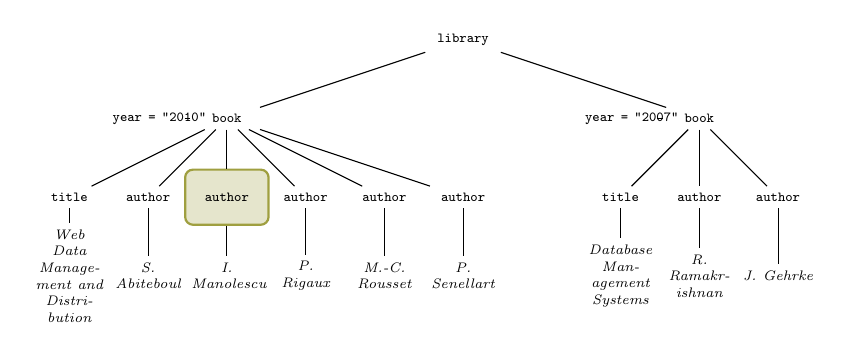
\begin{tikzpicture}[auto]
\tiny
  \tikzstyle{emptyStyle}=[text width=0.9cm, text centered]
  \tikzstyle{red}=[rounded corners=1mm,thick,draw=red!75,fill=red!20,text width=0.9cm, text centered]
  \tikzstyle{DarkViolet}=[rounded corners=1mm,thick,draw=DarkViolet!75,fill=DarkViolet!20,minimum size=7mm,text width=0.8cm, text centered]
  \tikzstyle{green}=[rounded corners=1mm,thick,draw=DarkOliveGreen!75,fill=DarkOliveGreen!20,minimum size=7mm,text width=0.8cm, text centered]
  \tikzstyle{cyan}=[rounded corners=1mm,thick,draw=DarkCyan!75,fill=DarkCyan!20,minimum size=7mm,text width=0.8cm, text centered]
 \tikzstyle{every label}=[black]
  \tikzstyle{HotPink}=[rounded corners=1mm,thick,draw=HotPink!75,fill=HotPink!20,minimum size=7mm,text width=0.8cm, text centered]
  \tikzstyle{noeudcourant}=[rounded corners=1mm,thick,draw=Olive!75,fill=Olive!20,minimum size=7mm,text width=0.9cm, text centered]
  \tikzstyle{indiaRed}=[rounded corners=1mm,thick,draw=indiaRed!75,fill=indiaRed!20,minimum size=7mm,text width=0.9cm, text centered]

  \begin{scope}
   % \node[emptyStyle](r) at (7,5) {Root};  
   %\node[emptyStyle](entete) at (3,4) {\texttt{$<?xml$ version $...>$}};
   %\draw[-] (r) -- (entete);
   \node[emptyStyle](library) at (7,4) {\verb?library?};
   % \draw[-] (r) -- (library);

    \node[emptyStyle](book1) at (4,3) {\verb?book?};
   \draw[-] (library) -- (book1);
   \node[emptyStyle](book2) at (10,3) {\verb?book?};
   \draw[-] (library) -- (book2);

    \node[emptyStyle](year1) at (3,3) {\verb?year = "2010"?};
   \draw[-] (book1) -- (year1);
    \node[emptyStyle](title1) at (2,2) {\verb?title?};
   \draw[-] (book1) -- (title1);
 \node[emptyStyle](texttitle1) at (2,1) {\it Web Data Management and Distribution};
   \draw[-] (title1) -- (texttitle1);
    \node[emptyStyle](author1) at (3,2) {\verb?author?};
   \draw[-] (book1) -- (author1);
   \node[emptyStyle](textauthor1) at (3,1) {\it S. Abiteboul};
   \draw[-] (author1) -- (textauthor1);
    \node[noeudcourant](author2) at (4,2) {\verb?author?};
   \draw[-] (book1) -- (author2);
   \node[emptyStyle](textauthor2) at (4,1) {\it I. Manolescu};
   \draw[-] (author2) -- (textauthor2);
    \node[emptyStyle](author3) at (5,2) {\verb?author?};
   \draw[-] (book1) -- (author3);
   \node[emptyStyle](textauthor3) at (5,1) {\it P. Rigaux};
   \draw[-] (author3) -- (textauthor3);
    \node[emptyStyle](author4) at (6,2) {\verb?author?};
   \draw[-] (book1) -- (author4);
   \node[emptyStyle](textauthor4) at (6,1) {\it M.-C. Rousset};
   \draw[-] (author4) -- (textauthor4);
    \node[emptyStyle](author5) at (7,2) {\verb?author?};
   \draw[-] (book1) -- (author5);
   \node[emptyStyle](textauthor5) at (7,1) {\it P. Senellart};
   \draw[-] (author5) -- (textauthor5);

    \node[emptyStyle](year2) at (9,3) {\verb?year = "2007"?};
   \draw[-] (book2) -- (year2);
    \node[emptyStyle](title2) at (9,2) {\verb?title?};
   \draw[-] (book2) -- (title2);
 \node[emptyStyle](texttitle2) at (9,1) {\it Database Management Systems};
   \draw[-] (title2) -- (texttitle2);
    \node[emptyStyle](author1prime) at (10,2) {\verb?author?};
   \draw[-] (book2) -- (author1prime);
   \node[emptyStyle](textauthor1prime) at (10,1) {\it R. Ramakrishnan};
   \draw[-] (author1prime) -- (textauthor1prime);
    \node[emptyStyle](author2prime) at (11,2) {\verb?author?};
   \draw[-] (book2) -- (author2prime);
   \node[emptyStyle](textauthor2prime) at (11,1) {\it J. Gehrke};
   \draw[-] (author2prime) -- (textauthor2prime);
\end{scope}
\end{tikzpicture}

\end{frame}

\begin{frame}{Quelques axes en exemple : Following}
\texttt{following}  : Selects everything in the document defined after the closing tag of the current node

\bigskip

\begin{tikzpicture}[auto]
\tiny
  \tikzstyle{emptyStyle}=[text width=0.9cm, text centered]
  \tikzstyle{red}=[rounded corners=1mm,thick,draw=red!75,fill=red!20,text width=0.9cm, text centered]
  \tikzstyle{DarkViolet}=[rounded corners=1mm,thick,draw=DarkViolet!75,fill=DarkViolet!20,minimum size=7mm,text width=0.8cm, text centered]
  \tikzstyle{green}=[rounded corners=1mm,thick,draw=DarkOliveGreen!75,fill=DarkOliveGreen!20,minimum size=7mm,text width=0.8cm, text centered]
  \tikzstyle{cyan}=[rounded corners=1mm,thick,draw=DarkCyan!75,fill=DarkCyan!20,minimum size=7mm,text width=0.8cm, text centered]
 \tikzstyle{every label}=[black]
  \tikzstyle{HotPink}=[rounded corners=1mm,thick,draw=HotPink!75,fill=HotPink!20,minimum size=7mm,text width=0.8cm, text centered]
  \tikzstyle{noeudcourant}=[rounded corners=1mm,thick,draw=Olive!75,fill=Olive!20,minimum size=7mm,text width=0.9cm, text centered]
  \tikzstyle{indiaRed}=[rounded corners=1mm,thick,draw=indiaRed!75,fill=indiaRed!20,minimum size=7mm,text width=0.9cm, text centered]

  \begin{scope}
   % \node[emptyStyle](r) at (7,5) {Root};  
   %\node[emptyStyle](entete) at (3,4) {\texttt{$<?xml$ version $...>$}};
   %\draw[-] (r) -- (entete);
   \node[emptyStyle](library) at (7,4) {\verb?library?};
   % \draw[-] (r) -- (library);

    \node[emptyStyle](book1) at (4,3) {\verb?book?};
   \draw[-] (library) -- (book1);
   \node[indiaRed](book2) at (10,3) {\verb?book?};
   \draw[-] (library) -- (book2);

    \node[emptyStyle](year1) at (3,3) {\verb?year = "2010"?};
   \draw[-] (book1) -- (year1);
    \node[emptyStyle](title1) at (2,2) {\verb?title?};
   \draw[-] (book1) -- (title1);
 \node[emptyStyle](texttitle1) at (2,1) {\it Web Data Management and Distribution};
   \draw[-] (title1) -- (texttitle1);
    \node[emptyStyle](author1) at (3,2) {\verb?author?};
   \draw[-] (book1) -- (author1);
   \node[emptyStyle](textauthor1) at (3,1) {\it S. Abiteboul};
   \draw[-] (author1) -- (textauthor1);
    \node[noeudcourant](author2) at (4,2) {\verb?author?};
   \draw[-] (book1) -- (author2);
   \node[emptyStyle](textauthor2) at (4,1) {\it I. Manolescu};
   \draw[-] (author2) -- (textauthor2);
    \node[indiaRed](author3) at (5,2) {\verb?author?};
   \draw[-] (book1) -- (author3);
   \node[indiaRed](textauthor3) at (5,1) {\it P. Rigaux};
   \draw[-] (author3) -- (textauthor3);
    \node[indiaRed](author4) at (6,2) {\verb?author?};
   \draw[-] (book1) -- (author4);
   \node[indiaRed](textauthor4) at (6,1) {\it M.-C. Rousset};
   \draw[-] (author4) -- (textauthor4);
    \node[indiaRed](author5) at (7,2) {\verb?author?};
   \draw[-] (book1) -- (author5);
   \node[indiaRed](textauthor5) at (7,1) {\it P. Senellart};
   \draw[-] (author5) -- (textauthor5);

    \node[indiaRed](year2) at (9,3) {\verb?year = "2007"?};
   \draw[-] (book2) -- (year2);
    \node[indiaRed](title2) at (9,2) {\verb?title?};
   \draw[-] (book2) -- (title2);
 \node[indiaRed](texttitle2) at (9,1) {\it Database Management Systems};
   \draw[-] (title2) -- (texttitle2);
    \node[indiaRed](author1prime) at (10,2) {\verb?author?};
   \draw[-] (book2) -- (author1prime);
   \node[indiaRed](textauthor1prime) at (10,1) {\it R. Ramakrishnan};
   \draw[-] (author1prime) -- (textauthor1prime);
    \node[indiaRed](author2prime) at (11,2) {\verb?author?};
   \draw[-] (book2) -- (author2prime);
   \node[indiaRed](textauthor2prime) at (11,1) {\it J. Gehrke};
   \draw[-] (author2prime) -- (textauthor2prime);
\end{scope}
\end{tikzpicture}

\end{frame}


%following-sibling
\subsection{Following-sibling}

 \begin{frame}{Quelques axes en exemple : Following-sibling}
\texttt{following-sibling} : Selects all siblings after the current node. \prof{sibling=frére ou s{\oe}ur}

\bigskip

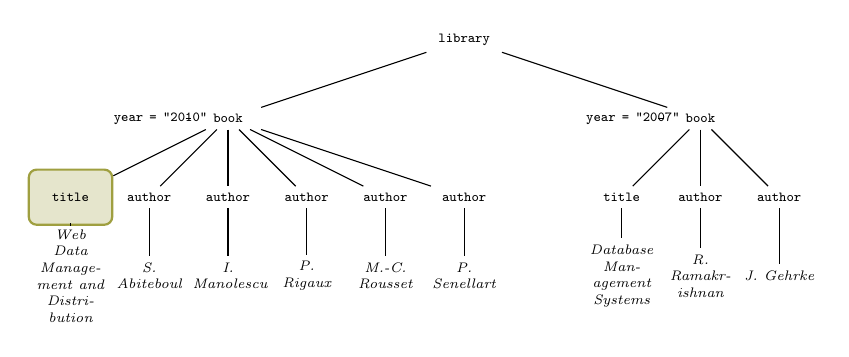
\begin{tikzpicture}[auto]
\tiny
  \tikzstyle{emptyStyle}=[text width=0.9cm, text centered]
  \tikzstyle{red}=[rounded corners=1mm,thick,draw=red!75,fill=red!20,text width=0.9cm, text centered]
  \tikzstyle{DarkViolet}=[rounded corners=1mm,thick,draw=DarkViolet!75,fill=DarkViolet!20,minimum size=7mm,text width=0.8cm, text centered]
  \tikzstyle{green}=[rounded corners=1mm,thick,draw=DarkOliveGreen!75,fill=DarkOliveGreen!20,minimum size=7mm,text width=0.8cm, text centered]
  \tikzstyle{cyan}=[rounded corners=1mm,thick,draw=DarkCyan!75,fill=DarkCyan!20,minimum size=7mm,text width=0.8cm, text centered]
 \tikzstyle{every label}=[black]
  \tikzstyle{HotPink}=[rounded corners=1mm,thick,draw=HotPink!75,fill=HotPink!20,minimum size=7mm,text width=0.8cm, text centered]
  \tikzstyle{noeudcourant}=[rounded corners=1mm,thick,draw=Olive!75,fill=Olive!20,minimum size=7mm,text width=0.9cm, text centered]
  \tikzstyle{indiaRed}=[rounded corners=1mm,thick,draw=indiaRed!75,fill=indiaRed!20,minimum size=7mm,text width=0.9cm, text centered]

  \begin{scope}
   % \node[emptyStyle](r) at (7,5) {Root};  
   %\node[emptyStyle](entete) at (3,4) {\texttt{$<?xml$ version $...>$}};
   %\draw[-] (r) -- (entete);
   \node[emptyStyle](library) at (7,4) {\verb?library?};
   % \draw[-] (r) -- (library);

    \node[emptyStyle](book1) at (4,3) {\verb?book?};
   \draw[-] (library) -- (book1);
   \node[emptyStyle](book2) at (10,3) {\verb?book?};
   \draw[-] (library) -- (book2);

    \node[emptyStyle](year1) at (3,3) {\verb?year = "2010"?};
   \draw[-] (book1) -- (year1);
    \node[noeudcourant](title1) at (2,2) {\verb?title?};
   \draw[-] (book1) -- (title1);
 \node[emptyStyle](texttitle1) at (2,1) {\it Web Data Management and Distribution};
   \draw[-] (title1) -- (texttitle1);
    \node[emptyStyle](author1) at (3,2) {\verb?author?};
   \draw[-] (book1) -- (author1);
   \node[emptyStyle](textauthor1) at (3,1) {\it S. Abiteboul};
   \draw[-] (author1) -- (textauthor1);
    \node[emptyStyle](author2) at (4,2) {\verb?author?};
   \draw[-] (book1) -- (author2);
   \node[emptyStyle](textauthor2) at (4,1) {\it I. Manolescu};
   \draw[-] (author2) -- (textauthor2);
    \node[emptyStyle](author3) at (5,2) {\verb?author?};
   \draw[-] (book1) -- (author3);
   \node[emptyStyle](textauthor3) at (5,1) {\it P. Rigaux};
   \draw[-] (author3) -- (textauthor3);
    \node[emptyStyle](author4) at (6,2) {\verb?author?};
   \draw[-] (book1) -- (author4);
   \node[emptyStyle](textauthor4) at (6,1) {\it M.-C. Rousset};
   \draw[-] (author4) -- (textauthor4);
    \node[emptyStyle](author5) at (7,2) {\verb?author?};
   \draw[-] (book1) -- (author5);
   \node[emptyStyle](textauthor5) at (7,1) {\it P. Senellart};
   \draw[-] (author5) -- (textauthor5);

    \node[emptyStyle](year2) at (9,3) {\verb?year = "2007"?};
   \draw[-] (book2) -- (year2);
    \node[emptyStyle](title2) at (9,2) {\verb?title?};
   \draw[-] (book2) -- (title2);
 \node[emptyStyle](texttitle2) at (9,1) {\it Database Management Systems};
   \draw[-] (title2) -- (texttitle2);
    \node[emptyStyle](author1prime) at (10,2) {\verb?author?};
   \draw[-] (book2) -- (author1prime);
   \node[emptyStyle](textauthor1prime) at (10,1) {\it R. Ramakrishnan};
   \draw[-] (author1prime) -- (textauthor1prime);
    \node[emptyStyle](author2prime) at (11,2) {\verb?author?};
   \draw[-] (book2) -- (author2prime);
   \node[emptyStyle](textauthor2prime) at (11,1) {\it J. Gehrke};
   \draw[-] (author2prime) -- (textauthor2prime);
\end{scope}
\end{tikzpicture}




\end{frame}


 \begin{frame}{Quelques axes en exemple : Following-sibling}
\texttt{following-sibling} : Selects all siblings after the current node

\bigskip

\begin{tikzpicture}[auto]
\tiny
  \tikzstyle{emptyStyle}=[text width=0.9cm, text centered]
  \tikzstyle{red}=[rounded corners=1mm,thick,draw=red!75,fill=red!20,text width=0.9cm, text centered]
  \tikzstyle{DarkViolet}=[rounded corners=1mm,thick,draw=DarkViolet!75,fill=DarkViolet!20,minimum size=7mm,text width=0.8cm, text centered]
  \tikzstyle{green}=[rounded corners=1mm,thick,draw=DarkOliveGreen!75,fill=DarkOliveGreen!20,minimum size=7mm,text width=0.8cm, text centered]
  \tikzstyle{cyan}=[rounded corners=1mm,thick,draw=DarkCyan!75,fill=DarkCyan!20,minimum size=7mm,text width=0.8cm, text centered]
 \tikzstyle{every label}=[black]
  \tikzstyle{HotPink}=[rounded corners=1mm,thick,draw=HotPink!75,fill=HotPink!20,minimum size=7mm,text width=0.8cm, text centered]
  \tikzstyle{noeudcourant}=[rounded corners=1mm,thick,draw=Olive!75,fill=Olive!20,minimum size=7mm,text width=0.9cm, text centered]
  \tikzstyle{indiaRed}=[rounded corners=1mm,thick,draw=indiaRed!75,fill=indiaRed!20,minimum size=7mm,text width=0.9cm, text centered]

  \begin{scope}
   % \node[emptyStyle](r) at (7,5) {Root};  
   %\node[emptyStyle](entete) at (3,4) {\texttt{$<?xml$ version $...>$}};
   %\draw[-] (r) -- (entete);
   \node[emptyStyle](library) at (7,4) {\verb?library?};
   % \draw[-] (r) -- (library);

    \node[emptyStyle](book1) at (4,3) {\verb?book?};
   \draw[-] (library) -- (book1);
   \node[emptyStyle](book2) at (10,3) {\verb?book?};
   \draw[-] (library) -- (book2);

    \node[emptyStyle](year1) at (3,3) {\verb?year = "2010"?};
   \draw[-] (book1) -- (year1);
    \node[noeudcourant](title1) at (2,2) {\verb?title?};
   \draw[-] (book1) -- (title1);
 \node[emptyStyle](texttitle1) at (2,1) {\it Web Data Management and Distribution};
   \draw[-] (title1) -- (texttitle1);
    \node[indiaRed](author1) at (3,2) {\verb?author?};
   \draw[-] (book1) -- (author1);
   \node[emptyStyle](textauthor1) at (3,1) {\it S. Abiteboul};
   \draw[-] (author1) -- (textauthor1);
    \node[indiaRed](author2) at (4,2) {\verb?author?};
   \draw[-] (book1) -- (author2);
   \node[emptyStyle](textauthor2) at (4,1) {\it I. Manolescu};
   \draw[-] (author2) -- (textauthor2);
    \node[indiaRed](author3) at (5,2) {\verb?author?};
   \draw[-] (book1) -- (author3);
   \node[emptyStyle](textauthor3) at (5,1) {\it P. Rigaux};
   \draw[-] (author3) -- (textauthor3);
    \node[indiaRed](author4) at (6,2) {\verb?author?};
   \draw[-] (book1) -- (author4);
   \node[emptyStyle](textauthor4) at (6,1) {\it M.-C. Rousset};
   \draw[-] (author4) -- (textauthor4);
    \node[indiaRed](author5) at (7,2) {\verb?author?};
   \draw[-] (book1) -- (author5);
   \node[emptyStyle](textauthor5) at (7,1) {\it P. Senellart};
   \draw[-] (author5) -- (textauthor5);

    \node[emptyStyle](year2) at (9,3) {\verb?year = "2007"?};
   \draw[-] (book2) -- (year2);
    \node[emptyStyle](title2) at (9,2) {\verb?title?};
   \draw[-] (book2) -- (title2);
 \node[emptyStyle](texttitle2) at (9,1) {\it Database Management Systems};
   \draw[-] (title2) -- (texttitle2);
    \node[emptyStyle](author1prime) at (10,2) {\verb?author?};
   \draw[-] (book2) -- (author1prime);
   \node[emptyStyle](textauthor1prime) at (10,1) {\it R. Ramakrishnan};
   \draw[-] (author1prime) -- (textauthor1prime);
    \node[emptyStyle](author2prime) at (11,2) {\verb?author?};
   \draw[-] (book2) -- (author2prime);
   \node[emptyStyle](textauthor2prime) at (11,1) {\it J. Gehrke};
   \draw[-] (author2prime) -- (textauthor2prime);
\end{scope}
\end{tikzpicture}

\end{frame}



\begin{frame}{Abréviations}

\textcolor{cyan}{\verb?child?} peut \^etre omis dans le chemin de localisation\\

\begin{flushright}
\textcolor{DarkViolet}{\verb?/inventory/drink/lemonade[child::amount>15]?}
\end{flushright}


\textcolor{cyan}{\verb?//a?} est une forme raccourcie de \textcolor{cyan}{\verb?/descendant-or-self::node()/child::a?}\\
\begin{flushright}
\textcolor{DarkViolet}{\verb?//lemonade[child::amount>15]?\\
\verb?/inventory//lemonade[child::amount>15]?}
\end{flushright}


\textcolor{cyan}{\verb?a//b?} est un raccourci pour \textcolor{cyan}{\verb?a/descendant-or-self::node()/child::b?}\\

\bigskip

\textcolor{cyan}{\verb?.?} est un raccourci pour \textcolor{cyan}{\verb?self::node()?}\\

\begin{flushright}
\textcolor{DarkViolet}{\verb?./inventory//lemonade[child::amount>15]?}
\end{flushright}

\textcolor{cyan}{\verb?..?} est un raccourci pour \textcolor{cyan}{\verb?parent::node()?}\\

\begin{flushright}
\textcolor{DarkViolet}{\verb?/inventory/drink/lemonade[child::amount>15]/../pop?}
\end{flushright}

\textcolor{cyan}{\verb?@attr\_name?} est un raccourci pour \textcolor{cyan}{\verb?attribute::attr\_name?}\\

\begin{flushright}
\textcolor{DarkViolet}{\verb?/inventory/drink/lemonade[@supplier='store']?}
\end{flushright}

\textcolor{cyan}{\verb?[1]?} est un raccourci pour \textcolor{cyan}{\verb?[position()=1]?}

\begin{flushright}
\textcolor{DarkViolet}{\verb?/inventory/drink[2]?}
\end{flushright}

\end{frame}

\begin{frame}[allowframebreaks]{Opérations et fonctions}

\begin{itemize}
\item XPath permet aussi d'effectuer des calculs des nombres, des booléens et des cha\^{i}nes de caractéres.

\item Opérations sur les nombres : \verb?+?, \verb?-? , \verb?*?, \verb?div?, \verb? mod?\\ \prof{Div au lieu de /, pourquoi ? Parce que / est un caractére spécial du langage utilisé pour les expressions de chemin
Modulo : le modulo est une fonction informatique qui au couple (a, b) d'entiers associe le reste r de la division euclidienne de a par b.}

Renvoie \verb?NaN? si l'un des arguments n'est pas un nombre. \prof{Not a Number}

\item Opérations sur les booléeans : \verb?and?, \verb?or?

\item égalité et différence (cha\^{i}nes de caractéres, nombres et booléens)  \verb?=?, \verb?!=? \prof{ex: \verb?@attr=1?}

\item Autres comparaisons (nombres seulement) : \verb?<?, \verb?<=?, \verb?>?, \verb?>= ?

\end{itemize}

\framebreak

{\bf Fonctions sur les ensembles de n{\oe}uds}
\begin{itemize}
\item \verb?count(nset)? nombre d'éléments dans l'ensemble de n{\oe}uds. 
\item \verb?name(nset)? nom du premier élément avec le préfixe de l'espace de noms
\item \verb?localname(nset)? nom du premier élément sans le préfixe de l'espace de noms
\item \verb?namespace-uri(nset)? préfixe de l'espace de noms du premier élément 
\item \verb?sum(nset)? somme des arguments de l'ensemble de n{\oe}uds (aprés conversion des cha\^{i}nes de caractéres en nombres).
\item \verb?position()? position dans le context
\item \verb?last()? nombre correspondant à la derniére position dans le context
\item \verb?id(mon\_id)? renvoi l'élément du document ayant pour identifiant \verb?mon\_id? (cherché parmis tous les attributs déclarés de type ID).
\end{itemize}

\begin{flushright}
\textcolor{DarkViolet}{\verb?//book[count(auteur)>=1]?\\
\verb?/biblio/book[position()=last()]?}
\end{flushright}

\framebreak

{\bf Fonctions sur les cha\^{i}nes de caractéres}

\begin{itemize}
\item \verb?concat(ch1, ..., chn)?, \verb?starts-with(ch1,ch2)?, \verb?contains(ch1,ch2)?, \verb?substring-before(ch1,ch2)?, \verb?substring-after(ch1,ch2)?, \verb?substring(ch,i,l)?, \verb?string-length(ch)?, \verb?normalize-space(ch)?, \verb?translate(ch1,ch2,ch3)?
\end{itemize}

\begin{flushright}
\textcolor{DarkViolet}{\verb?//titre[contains(text(),"Star")]?}
\end{flushright}

\prof{Exemple substring : extraire le ISBN 10  partir du ISBN 13.}

Voir \url{http://www.w3.org/TR/xpath\#section-Function-Calls}


\framebreak

{\bf Fonctions sur les booléens}

\begin{itemize}
\item \verb?not(bool)?
\end{itemize}

\begin{flushright}
\textcolor{DarkViolet}{\verb?not(@attr = 1)?\\
\verb?not(not(@attr = 1) or false()) and true()?\\
\verb?//book[not(count(auteur)>=1)]?
}
\end{flushright}


\framebreak

{\bf Fonctions sur les nombres}

\begin{itemize}
\item \verb?floor(n)? arrondi à l'entier supérieur de n
\item \verb?ceiling(n)? arrondi à l'entier inférieur de n
\item \verb?round(n)? arrondi entier de \verb?n? (plus proche de \verb?floor(n)? ou \verb?ceiling(n)?)
\end{itemize}

Voir \url{http://www.w3.org/TR/xpath\#section-Function-Calls}

\end{frame}


\begin{frame}{Zoom sur les espaces de noms}

\texttt{
<\textcolor{cyan}{html} xmlns="\textcolor{orange}{http://www.w3.org/1999/xhtml}">
</\textcolor{cyan}{html}>
}

\bigskip

Deux fonctions :\\
\textcolor{cyan}{local-name}\\
\textcolor{orange}{namespace-uri}\\

\bigskip

Utilisation (exemples) :\\
\verb?//*[local-name()='html']?\\
\verb?//*[namespace-uri()='http://www.w3.org/1999/xhtml'?\\
\verb?//*[local-name()='html']/namespace-uri()?\\

\end{frame}


\begin{frame}[allowframebreaks]{Zoom sur le cas des \texttt{ID} et \texttt{IDREF(S)}}

Fonctions :\\
id\\
idref\\

\bigskip

Utilisation (exemple) :\\

\verb?//id("0-201-53771-0")/child::author?	retourne les auteurs de l'élément dont l'ID est "0-201-53771-0"\\

\medskip

\verb?/library/document[3]/id(@references)/titre? retourne les titres des documents référencés (references est un IDREFS) par le troisième document\\

\medskip

\verb?//idref("0-201-53771-0")?	retourne tous les éléments qui référencent "0-201-53771-0"

\framebreak


\begin{center}
\figSized{images/exID1.jpg}{Fichier contenant des ID}{1}
\end{center}

\framebreak


\begin{center}
\figSized{images/exID2.jpg}{Requ\^ete avec fonction ID}{1}
\end{center}

\end{frame}

\begin{frame}{XPath 2.0}

 \begin{itemize}
 \item Repose toujours sur la notion de chemin de localisation afin de naviguer dans le document XML.
\item Pas juste une extension de XPath 1.0, c'est une véritable refonte de XPath : une fusion entre XPath 1.0 et XQuery.
\item Caractéristiques :
\begin{itemize}
\item Support de 19 types prédéfinis (date, etc), avec test de type ;
\item Réponse = séquence ordonnée de valeurs (et plus un NodeSet) ; \prof{ordonnée et autorisant les doublons à la place d'ensembles}
\item Opérateur d'intersection, union et except ;
\item Opérateurs de quantification ;
\item Boucles, tri, définition interne (let) ;
\item Expressions conditionnelles (if-then-else) ;
\item Extensible (possibilité de créer des fonctions utilisateurs).
\end{itemize}
 \end{itemize}

 $\Rightarrow$ Un sous-language de XQuery que nous verrons dans la suite du cours
 \prof{ nouveau node tests : attribute()
 nested path expression : tout expressions renvoyé un path expression peut \^etre utilisée comme un pas. Ex : /book/(author | editor)/name
 }

\end{frame}

%\nocite{WDMD,ABS99,Bri07,XML_nut,Mich99,w3c,W3Schools}

% \begin{frame}[allowframebreaks]{Références}

% \begin{thebibliography}{8}
% \bibitem[ABS99]{ABS99}
% Serge Abiteboul, Peter Buneman, and Dan Suciu.
% \newblock {\em {Data on the Web: From Relations to Semistructured Data and
%   XML}}.
% \newblock Morgan Kaufmann, 1999.

% \bibitem[AMR04]{WDMD}
% Serge Abiteboul, Ioana Manolescu, Philippe Rigaux, Marie-Christine Rousset, and
%   Pierre Senellart.
% \newblock {\em {\textbf{Web Data Management and Distribution}}}.
% \newblock à paraitre, consulter le site de Philippe Rigaux
%   (\url{http://cedric.cnam.fr/~rigaux}) pour un accés au matériel mis à
%   disposition pour le cours NFE204.

% \bibitem[Bri07]{Bri07}
% Alexandre Briant.
% \newblock {\em {XML - Cours et exercices}}.
% \newblock Eyrolles, 2007.

% \bibitem[HM04]{XML_nut}
% Elliotte~R. Harold and Scott~W. Means.
% \newblock {\em XML in a Nutshell, Third Edition}.
% \newblock {O'Reilly Media, Inc.}, 2004.

% \bibitem[Mic99]{Mich99}
% Alain Michard.
% \newblock {\em {XML, langage et applications}}.
% \newblock Eyrolles, 1999.

% \bibitem[W3C]{w3c}
% {Site du World Wide Web Consortium}.
% \newblock \url{w3c.org}.

% \bibitem[W3S]{W3Schools}
% {Site W3 Schools}.
% \newblock \url{www.w3schools.com/}.

% \bibitem[W3Cd]{w3c/xpath}
% {Site du World Wide Web Consortium, XPath}.
% \newblock \url{http://www.w3.org/TR/xpath}.

% \end{thebibliography}
% \end{frame